% \iffalse meta-comment
%
% Copyright (C) 2017- by Yanshuo Chu <yanshuoc@gmail.com>
%
% This file may be distributed and/or modified under the
% conditions of the LaTeX Project Public License, either version 1.3a
% of this license or (at your option) any later version.
% The latest version of this license is in:
%
% http://www.latex-project.org/lppl.txt
%
% and version 1.3a or later is part of all distributions of LaTeX
% version 2004/10/01 or later.
%
% \fi
%
% \iffalse
%<*driver>
\ProvidesFile{hithesis.dtx}[2017/03/26 0.0.1 Harbin Institute of Technology Thesis Template]
\documentclass{ltxdoc}
\usepackage{dtx-style}

\EnableCrossrefs
\CodelineIndex
\RecordChanges

\begin{document}
  \DocInput{\jobname.dtx}
\end{document}
%</driver>
% \fi
%
% \CheckSum{0}
%
% \CharacterTable
%  {Upper-case    \A\B\C\D\E\F\G\H\I\J\K\L\M\N\O\P\Q\R\S\T\U\V\W\X\Y\Z
%   Lower-case    \a\b\c\d\e\f\g\h\i\j\k\l\m\n\o\p\q\r\s\t\u\v\w\x\y\z
%   Digits        \0\1\2\3\4\5\6\7\8\9
%   Exclamation   \!     Double quote  \"     Hash (number) \#
%   Dollar        \$     Percent       \%     Ampersand     \&
%   Acute accent  \'     Left paren    \(     Right paren   \)
%   Asterisk      \*     Plus          \+     Comma         \,
%   Minus         \-     Point         \.     Solidus       \/
%   Colon         \:     Semicolon     \;     Less than     \<
%   Equals        \=     Greater than  \>     Question mark \?
%   Commercial at \@     Left bracket  \[     Backslash     \\
%   Right bracket \]     Circumflex    \^     Underscore    \_
%   Grave accent  \`     Left brace    \{     Vertical bar  \|
%   Right brace   \}     Tilde         \~}
%
% \DoNotIndex{\newenvironment,\@bsphack,\@empty,\@esphack,\sfcode}
% \DoNotIndex{\addtocounter,\label,\let,\linewidth,\newcounter}
% \DoNotIndex{\noindent,\normalfont,\par,\parskip,\phantomsection}
% \DoNotIndex{\providecommand,\ProvidesPackage,\refstepcounter}
% \DoNotIndex{\RequirePackage,\setcounter,\setlength,\string,\strut}
% \DoNotIndex{\textbackslash,\texttt,\ttfamily,\usepackage}
% \DoNotIndex{\begin,\end,\begingroup,\endgroup,\par,\\}
% \DoNotIndex{\if,\ifx,\ifdim,\ifnum,\ifcase,\else,\or,\fi}
% \DoNotIndex{\let,\def,\xdef,\edef,\newcommand,\renewcommand}
% \DoNotIndex{\expandafter,\csname,\endcsname,\relax,\protect}
% \DoNotIndex{\Huge,\huge,\LARGE,\Large,\large,\normalsize}
% \DoNotIndex{\small,\footnotesize,\scriptsize,\tiny}
% \DoNotIndex{\normalfont,\bfseries,\slshape,\sffamily,\interlinepenalty}
% \DoNotIndex{\textbf,\textit,\textsf,\textsc}
% \DoNotIndex{\hfil,\par,\hskip,\vskip,\vspace,\quad}
% \DoNotIndex{\centering,\raggedright,\ref}
% \DoNotIndex{\c@secnumdepth,\@startsection,\@setfontsize}
% \DoNotIndex{\ ,\@plus,\@minus,\p@,\z@,\@m,\@M,\@ne,\m@ne}
% \DoNotIndex{\@@par,\DeclareOperation,\RequirePackage,\LoadClass}
% \DoNotIndex{\AtBeginDocument,\AtEndDocument}
%
% \GetFileInfo{\jobname.dtx}
%
%
% \def\indexname{索引}
% \def\glossaryname{修改记录}
% \IndexPrologue{\section{\indexname}}
% \GlossaryPrologue{\section{\glossaryname}}
%
% \title{\bfseries\color{violet}\hithesis:哈尔滨工业大学学位论文模板}
% \author{{\fangsong 初砚硕}\\[5pt]\texttt{yanshuoc@gmail.com}}
% \date{v\fileversion\ (\filedate)}
% \maketitle\thispagestyle{empty}
%
% \begin{abstract}\noindent
% 该宏包为哈尔滨工业大学本、硕、博毕业论文模板。以后会陆续加入开题、中期、博士后
% 出站报告等模板。
% \end{abstract}
%
% \vskip2cm
% \def\abstractname{免责声明}
% \begin{abstract}
% \noindent
% \begin{enumerate}
% \item 本模板的发布遵守 \LaTeX\ Project Public License,使用前请认真阅读协议内
%   容。
% \item 本模板为作者根据\hit 教务处颁发的\UGR ,\hit 研究生院颁发的\PGR 编写而成
% ,为方便\hit 学生撰写毕业论文使用。
% \item \hit 教务处和研究生院只提供毕业论文写作指南,不提供官方模板(包括MS word
% ),也不会授权第三方模板为官方模板,所以此模板仅为写作指南的参考实现,不保证格
% 式审查老师不提意见。任何由于使用本模板而引起的论文格式审查问题均与本模板作者无
% 关。
% \item 任何个人或组织以本模板为基础进行修改、扩展而生成的新的专用模板,请严格遵
%   守 \LaTeX\ Project Public License 协议。由于违犯协议而引起的任何纠纷争端均与
%   本模板作者无关。
% \end{enumerate}
% \end{abstract}
%
%
% \clearpage
% \pagestyle{fancy}
% \begin{multicols}{2}[
%   \setlength{\columnseprule}{.4pt}
%   \setlength{\columnsep}{18pt}]
%   \tableofcontents
% \end{multicols}
% \clearpage
%
% \section{模板介绍}
% \hithesis\ (\textbf{H}arbin\textbf{I}nstitute of \textbf{T}echnology \LaTeX\
% \textbf{Thesis} Template) 是为了帮助\hit 毕业生撰写毕业论文而编写
% 的 \LaTeX\ 论文模板。
%
% 本文档将尽量完整的介绍模板的使用方法,如有不清楚之处可以参考示例文档或者根据
% 第~\ref{sec:howtoask} 节说明提问,有兴趣者都可以参与完善此手册,也非常欢迎对代
% 码的贡献。
%
% \note[注意:]{模板的作用在于减少论文写作过程中格式调整的时间。前提是遵守模板的
% 用法,否则即便用了 \hithesis\ 也难以保证输出的论文符合学校规范。}
%
%
% \section{安装}
% \label{sec:installation}
% 未来
% \hithesis\ 将已经包含在主要的 \TeX\ 发行版中,一般不需要安装,可以利用发行版自
% 带更新工具自动更新。阅读文档可以使用以下命令:
% \begin{shell}
% $ texdoc hithesis
% \end{shell}
%
% 如果要使用开发版,需自己下载,\hithesis\ 相关链接:
% \begin{itemize}
% \item github:\href{https://gihitb.com/dustincys/hithesis}
% {https://gihitb.com/dustincys/hithesis}
% \item oschina:\href{https://git.oschina.net/dustincys/hithesis}
% {https://git.oschina.net/dustincys/hithesis}
% \end{itemize}
%
% \note[注意:]{如果登录不了github的同学可以登录oschina下载。}
%
% \subsection{模板的组成}
% 下表列出了 \hithesis\ 的主要文件及其功能介绍:
%
% \begin{longtable}{l|p{8cm}}
% \toprule
% {\heiti 文件(夹)} & {\heiti 功能描述}\\\midrule
% \endfirsthead
% \midrule
% {\heiti 文件(夹)} & {\heiti 功能描述}\\\midrule
% \endhead
% \endfoot
% \endlastfoot
% hithesis.ins & \textsc{DocStrip} 驱动文件(开发用) \\
% hithesis.dtx & \textsc{DocStrip} 源文件(开发用)\\\midrule
% hithesis.cls & 模板类文件\\
% hithesis.cfg & 模板配置文件\\
% hithesis.bst & 参考文献样式文件\\\midrule
% hithesis.ist & 索引样式文件\\\midrule
% reference.bib & 文档参考文献\\
% main.tex & 示例文档主文件\\
% front/ & 正文之前内容\\
% body/ & 正文内容\\
% body/ & 正文之后内容\\
% figures/ & 示例文档图片路径\\
% hithesis.sty & 为示例文档加载其它宏包\\\midrule
% Makefile & Makefile\\
% latexmkrc & latexmk 配置文件 \\
% README.md & Readme\\
% \textbf{hithesis.pdf} & 用户手册(本文档)\\\bottomrule
% \end{longtable}
%
% 几点说明:
% \begin{itemize}
% \item \file{hithesis.cls} 和 \file{hithesis.cfg} 可由 \file{hithesis.ins}
%   和 \file{hithesis.dtx} 生成,但为了降低新手用户的使用难度,故
%   将 \file{hithesis.cls} 和 \file{hithesis.cfg} 文件一起发布。
% \item 使用前阅读文档:\file{hithesis.pdf}。
% \end{itemize}
%
% \subsection{生成模板}
% \label{sec:generate-cls}
% \note[提示:]{若使用 \TeX 发行版自带的 \hithesis\ 或 Gihitb/OSChina
% 上发布的版本,可忽略此节,直接阅读第~\ref{sec:generate-thesis}节。若下载
% CTAN 包或者 Gihitb/OSChina 开发代码,请阅读本节了解生成模板文件的步骤。}
%
% 模板解压缩后生成文件夹 \file{hithesis-vX.Y.Z}\footnote{\texttt{vX.Y.Z} 为版本号。},
% 其中包括:模板源文件(\file{hithesis.ins} 和 \file{hithesis.dtx}),参考文献
% 样式 \file{hithesis.bst},示例文档
% (\file{main.tex},\file{shuji.tex},\file{hithesis.sty}\footnote{可能用到的包
% 以及一些命令定义都放在这里,以免 \file{hithesis.cls} 过分臃
% 肿。},\file{data/} 和 \file{figures/} 和 \file{ref/})。在使用之前需要先生成模
% 板文件和配置文件(具体命令细节请参考 \file{README.md} 和 \file{Makefile}):
%
% \begin{shell}
% $ cd hithesis-vX.Y.Z
% # 生成 hithesis.cls 和 hithesis.cfg
% $ latex hithesis.ins
%
% # 下面的命令用来生成用户手册,可以不执行
% $ xelatex hithesis.dtx
% $ makeindex -s gind.ist -o hithesis.ind hithesis.idx
% $ makeindex -s gglo.ist -o hithesis.gls hithesis.glo
% $ xelatex hithesis.dtx
% $ xelatex hithesis.dtx  % 生成说明文档 hithesis.pdf
% \end{shell}
%
% \subsection{生成论文}
% \label{sec:generate-thesis}
% 本节介绍几种常见的生成论文的方法。用户可根据自己的情况选择。
%
% \subsubsection{\XeLaTeX}
% \label{sec:xelatex}
% 很多用户对 \LaTeX\ 命令执行的次数不太清楚。一个基本的原则是多次运行 \LaTeX\ 命
% 令直至不再出现警告。下面给出生成示例文档的详细过程(\texttt{\#} 开头的行为注
% 释),首先来看推荐的 \texttt{xelatex} 方式:
% \begin{shell}
% # 1. 发现里面的引用关系,文件后缀 .tex 可以省略
% $ xelatex main
%
% # 2. 编译参考文件源文件,生成 bbl 文件
% $ bibtex main
%
% # 3. 下面解决引用
% $ xelatex main
% $ xelatex main   # 如果不需要生成索引此时生成完整的 pdf 文件
% $ splitindex main -- -s hithesis.ist  # 自动生成索引
% $ xelatex main.tex
% \end{shell}
%
% \subsubsection{latexmk}
% \label{sec:latexmk}
% \texttt{latexmk} 命令支持全自动生成 \LaTeX\ 编写的文档,并且支持使用不同的工具
% 链来进行生成,它会自动运行多次工具直到交叉引用都被解决。下面给出了一个用
% \texttt{latexmk} 调用 \texttt{xelatex} 生成最终文档的示例:
% \begin{shell}
% # 一句话就够了!
% $ latexmk -xelatex main
% \end{shell}
%
% \subsubsection{make}
% \label{sec:make}
% \note[提示:]{若要使用 \texttt{make} 编译,需自行下载模板。因为 \TeX\ 发行版中
% 的 \file{Makefile} 不在当前目录。}
%
% 上面的方法虽然不复杂,但是每次都输入还是非常罗嗦,所以 \hithesis\ 提供了一
% 个 \file{Makefile}:
%
% \begin{shell}
% $ make clean
% $ make cls       # 生成 hithesis.cls 和 hithesis.cfg
% $ make doc       # 生成说明文档 hithesis.pdf
% $ make thesis    # 生成示例文档 main.pdf
% \end{shell}
%
% \hithesis\ 的 \file{Makefile} 默认用 \texttt{latexmk} 调用\texttt{xelatex} 编
% 译,此外还支持直接用 \texttt{xelatex} 编译。如有需要可修
% 改 \file{Makefile} 开头的参数或通过命令行传递参数(请参看 \file{README.md}),
% 进一步还可以修改 \file{latexmkrc} 进行定制。
%
% \subsection{升级}
% \label{sec:updgrade}
% \hithesis\ 升级非常简单,可以通过 \TeX 发行版的包管理工具自动更新发行版,也可
% 以下载最新的开发版,
% 将 \file{hithesis.ins},\file{hithesis.dtx} 拷贝至工作目
% 录覆盖相应的文件,然后运行:
% \begin{shell}
% $ latex hithesis.ins
% \end{shell}
%
% 生成新的类文件和配置文件即可。也可以直接拷
% 贝 \file{hithesis.cls},\file{hithesis.cfg} 和
% \file{hithesis.ist},免去上面命令的执行。
%
%
% \section{使用说明}
% \label{sec:usage}
% 本手册假定用户已经能处理一般的 \LaTeX\ 文档,并对 \BibTeX\ 有一定了解。如果
% 从来没有接触过 \TeX\ 和 \LaTeX,建议先学习相关的基础知识。
%
% \subsection{关于提问}
% \label{sec:howtoask}
% 按照优先级推荐提问的位置如下:
%
% \begin{itemize}
% \item \href{http://gihitb.com/dustincys/hithesis/issues}{Gihitb Issues}
% \item \href{https://git.oschina.net/dustincys/hithesis/issues}{OSChina Issues}
% \item hithesis QQ 讨论群:259959600
% \end{itemize}
%
% \subsection{示例文件}
% \label{sec:userguide}
% 模板核心文件有三
% 个:\file{hithesis.cls},\file{hithesis.cfg} 和\file{hithesis.bst},但是如果
% 没有示例文档用户会发现很难下手。所以推荐新用户从模板自带的示例文档入手,里面包
% 括了论文写作用到的所有命令及其使用方法,只需要用自己的内容进行相应替换就可以。
% 对于不清楚的命令可以查阅本手册。下面的例子描述了模板中章节的组织形式,来自于示
% 例文档,具体内容可以参考模板附带的 \file{main.tex}。
%
% \lstinputlisting[style=lstStyleLaTeX]{main.tex}
%
% \subsection{论文选项}
% \label{sec:option}
%
% 论文选项,就是在\file{main.tex}文件的开头,非注释的第一行的方括号中填写的选项,示例见上节。
% 各个选项的含义说明已经在上节中说明,所以这里就不重复了。
%
% \subsection{中文字体}
% \label{sec:chinese-fonts}
% 正确配置中文字体是使用模板的第一步。模板调用 \CTeX\ 宏包,只提供基于
% \pkg{xeCJK} 包,使用 \XeLaTeX\ 编译的方式。
% 关于如何使用字体命令、字号等等,属于模板格式范畴,在实现细节中讨论。
% 关于中文字体安装、配置的所有问题不在本模板讨论 范围。
%
% \subsection{前文}
% \label{sec:titlepage}
% 前文内容是正文之前,含封面、摘要、目录、符号表。
% 封面信息提供两种配置方法:一是通过统一设置命 令 \cs{hitsetup}
% 通过\emph{key=value} 形式完成;二是每个信息利用命令独立设置, 其中命令的名字跟
% \emph{key} 相同。两种方式可以交叉使用,并按顺序执行(即后来的设置会覆
% 盖前面的)。以 \texttt{c} 开头的命令跟中文相关,\texttt{e}
% 开头则为对应的英文。
%
% \DescribeMacro{\hitsetup}
% \cs{hitsetup} 用法与常见 \emph{key=value} 命令相同,如下:
% \begin{latex}
% \hitsetup{
%   key1 = value1,
%   key2 = {a value, with comma},
% }
% % 可以多次调用
% \hitsetup{
%   key3 = value3,
%   key1 = value11, % 覆盖 value1
% }
% \end{latex}
%
% \note[注意:]{\cs{hitsetup} 使用 \pkg{kvoptions} 机制,所以配置项之间不能有空行,否则
% 会报错。}
%
% 大多数命令的使用方法都是: \cs{command}\marg{arg},例外者将具体指出。这些命令都
% 在示例文档的 \file{front/cover.tex} 中。
%
% \subsubsection{密级}
% \label{sec:setup-secret}
% \DescribeMacro{statesecrets}
% \DescribeMacro{natclassifiedindex}
% \DescribeMacro{intclassifiedindex}
% 定义秘密级别和国内国际索引号。
% \begin{latex}
% \hitsetup{
% statesecrets={公开},
% natclassifiedindex={TM301.2},
% intclassifiedindex={62-5},
% }
% \end{latex}
%
% \subsubsection{论文标题}
% \myentry{论文标题}
% \DescribeMacro{ctitle}
% \DescribeMacro{etitle}
% \DescribeMacro{ctitleone}
% \DescribeMacro{ctitletwo}
% \DescribeMacro{csubtitle}
% \DescribeMacro{esubtitle}
% 中英文标题。
% 如果有副标题,需要在封面选项中设置subtitle=true,否则不显示副标题。
% \begin{latex}
% \hitsetup{
%   ctitle={论文中文题目},
%   etitle={Thesis English Title},
%   csubtitle={论文中文副题目(如果有)},
%   esubtitle={Thesis English Sub-Title (if necessary)},
%   ctitleone={本科生论文中文题目上部分},
%   ctitletwo={本科生论文中文题目下部分},
% }
% \end{latex}
%
% \subsubsection{作者姓名}
% \myentry{作者姓名}
% \DescribeMacro{cauthor}
% \DescribeMacro{eauthor}
% 作者姓名。
% \begin{latex}
% \hitsetup{
%   cauthor={中文姓名},
%   eauthor={Name in Pinyin}
% }
% \end{latex}
%
% \subsubsection{申请学位名称}
% \label{sec:degree}
% \myentry{学科名称}
% \DescribeMacro{cxueke}
% \DescribeMacro{exueke}
% 按照入学的培养计划中学科自行填写,具体学科名称不是本文档范畴。
%
% \begin{latex}
% \hitsetup{
%   cxueke={工学},
%   exueke={Engineering},
% }
% \end{latex}
%
% \subsubsection{院系名称}
% \myentry{院系名称}
% \DescribeMacro{caffil}
% \DescribeMacro{eaffil}
% 院系名称,同上,按照入学的培养计划中学科自行填写,具体院系名称不是本文档范畴。
% \begin{latex}
% \hitsetup{
%  caffil={机电工程学院},
%  eaffil={\emultiline[t]{School of Mechatronics Engineering \\ Mechatronics Engineering}},
% }
% \end{latex}
% \note[注意:]{个别学院英文名过长,使用以上方法自行换行。}
%
% \subsubsection{专业名称}
% \myentry{专业名称}
% \DescribeMacro{csubject}
% \DescribeMacro{esubject}
% 专业名称,同上,按照入学的培养计划中学科自行填写,具体名称不是本文档范畴。
% \begin{latex}
% \hitsetup{
%  csubject={机械制造及其自动化},
%  esubject={Computer Science and Technology},
% }
% \end{latex}
%
% \subsubsection{导师}
% \myentry{导师}
% \DescribeMacro{csupervisor}
% \DescribeMacro{esupervisor}
% 直接导师。
% \begin{latex}
% \hitsetup{
%   csupervisor={导师~教授},
%   esupervisor={Supervisor}
% }
% \end{latex}
%
% \myentry{副导师}
% \DescribeMacro{cassosupervisor}
% \DescribeMacro{eassosupervisor}
% 副指导教师。
% \begin{latex}
% \hitsetup{
%   cassosupervisor={副导师~副教授},
%   eassosupervisor={2nd Boss}
% }
% \end{latex}
%
% \myentry{联合导师}
% \DescribeMacro{ccosupervisor}
% \DescribeMacro{ecosupervisor}
% 硕士生联合指导教师,博士生联合导师。
% \begin{latex}
% \hitsetup{
%   ccosupervisor={联合导师~教授},
%   ecosupervisor={3rd Boss}
% }
% \end{latex}
%
% \subsubsection{成文日期}
% \myentry{日期}
% \DescribeMacro{cdate}
% \DescribeMacro{edate}
% 默认为当前时间,也可以自己指定。
% \begin{latex}
% \hitsetup{
%   cdate={中文日期},
%   edate={English Date},
% }
% \end{latex}
%
% \subsubsection{学生类型}
% \myentry{学生类型}
% \DescribeMacro{cstudenttype}
% \DescribeMacro{estudenttype}
% 非全日制教育申请学位者
%(同等学力人员)、(工程硕士)、(工商管理硕士)、
%(高级管理人员工商管理硕士)、(公共管理硕士)、(中职教师)、(高校教师)等,
% 具体要求按照入学的培养计划中学科自行填写,具体名称不是本文档范畴。
% \begin{latex}
% \hitsetup{
%   cstudenttype={同等学力人员},
%   estudenttype={Master of Art},
% }
% \end{latex}
%
% \subsubsection{学号}
% \myentry{学号}
% \DescribeMacro{cstudentid}
% 学号,具体要求按照入学的培养计划中学科自行填写。
% \begin{latex}
% \hitsetup{
%   cstudentid={9527},
% }
% \end{latex}
%
% \subsubsection{摘要}
% \myentry{摘要正文}
% \DescribeEnv{cabstract}
% \DescribeEnv{eabstract}
% \note[说明:]{摘要正文只能用环境命令的形式,不支持 \cs{hitsetup}。}
%
% \begin{latex}
% \begin{cabstract}
%  摘要请写在这里...
% \end{cabstract}
%
% \begin{eabstract}
%  Here comes the abstract in English...
% \end{eabstract}
% \end{latex}
%
% \myentry{关键词}
% \DescribeMacro{ckeywords}
% \DescribeMacro{ekeywords}
% 关键词用英文逗号分割写入相应的命令中,模板会解析各关键词并生成符合不同论文格式
% 要求的关键词格式。
% \begin{latex}
% \hitsetup{
%   ckeywords={关键词 1, 关键词 2},
%   ekeywords={keyword 1, keyword 2}
% }
% \end{latex}
%
% \subsubsection{符号对照表}
% \DescribeEnv{denotation}
% 主要符号表环境,单独在文件\file{front/denotation.tex}中。
% 跟据\PGR\
% 示例中要求,我工符号表是table环境,示例文件如下,由于我工要求博士论文图表标题是双语,所以任何对单个标题的全局格式调整都会影响到双语标题,所以这里使用\cs{vspace},具体见实现细节中的描述。
% \begin{latex}
% \begin{denotation}
% \begin{table}[h]%此处最好是h
% \caption{国际单位制中具有专门名称的导出单位}
% \vspace{0.5em}\centering\wuhao
% \begin{tabular}{ccccc}
% \toprule[1.5pt]
% 量的名称&单位名称&单位符号&其它表示实例\\
% \midrule[1pt]
% 频率&赫[兹]&Hz&s-1\\
% \bottomrule[1.5pt]
% \end{tabular}
% \end{table}
% \end{denotation}
% \end{latex}
%
% \subsubsection{目录}
% 目录不需要用户干预,自动生成,具体命令已经写在\file{main.tex}中。
%
% \subsection{正文}
%
% \subsubsection{图和表}
% \hit\ 博士毕业论文要求使用中英双语图题、表题,这增加了维护难度。
% 因为现有唯一的方法是在已有的图题或表题的基础上再添加一行英语图题或表题。
% 两个题之间的距离具体多少不在\PGR\ 中要求。目前的方法是用户手动调节该距离。
% 单张双语图题的格式如下,
% \begin{latex}
% \begin{figure}[htpb]
% \centering
% 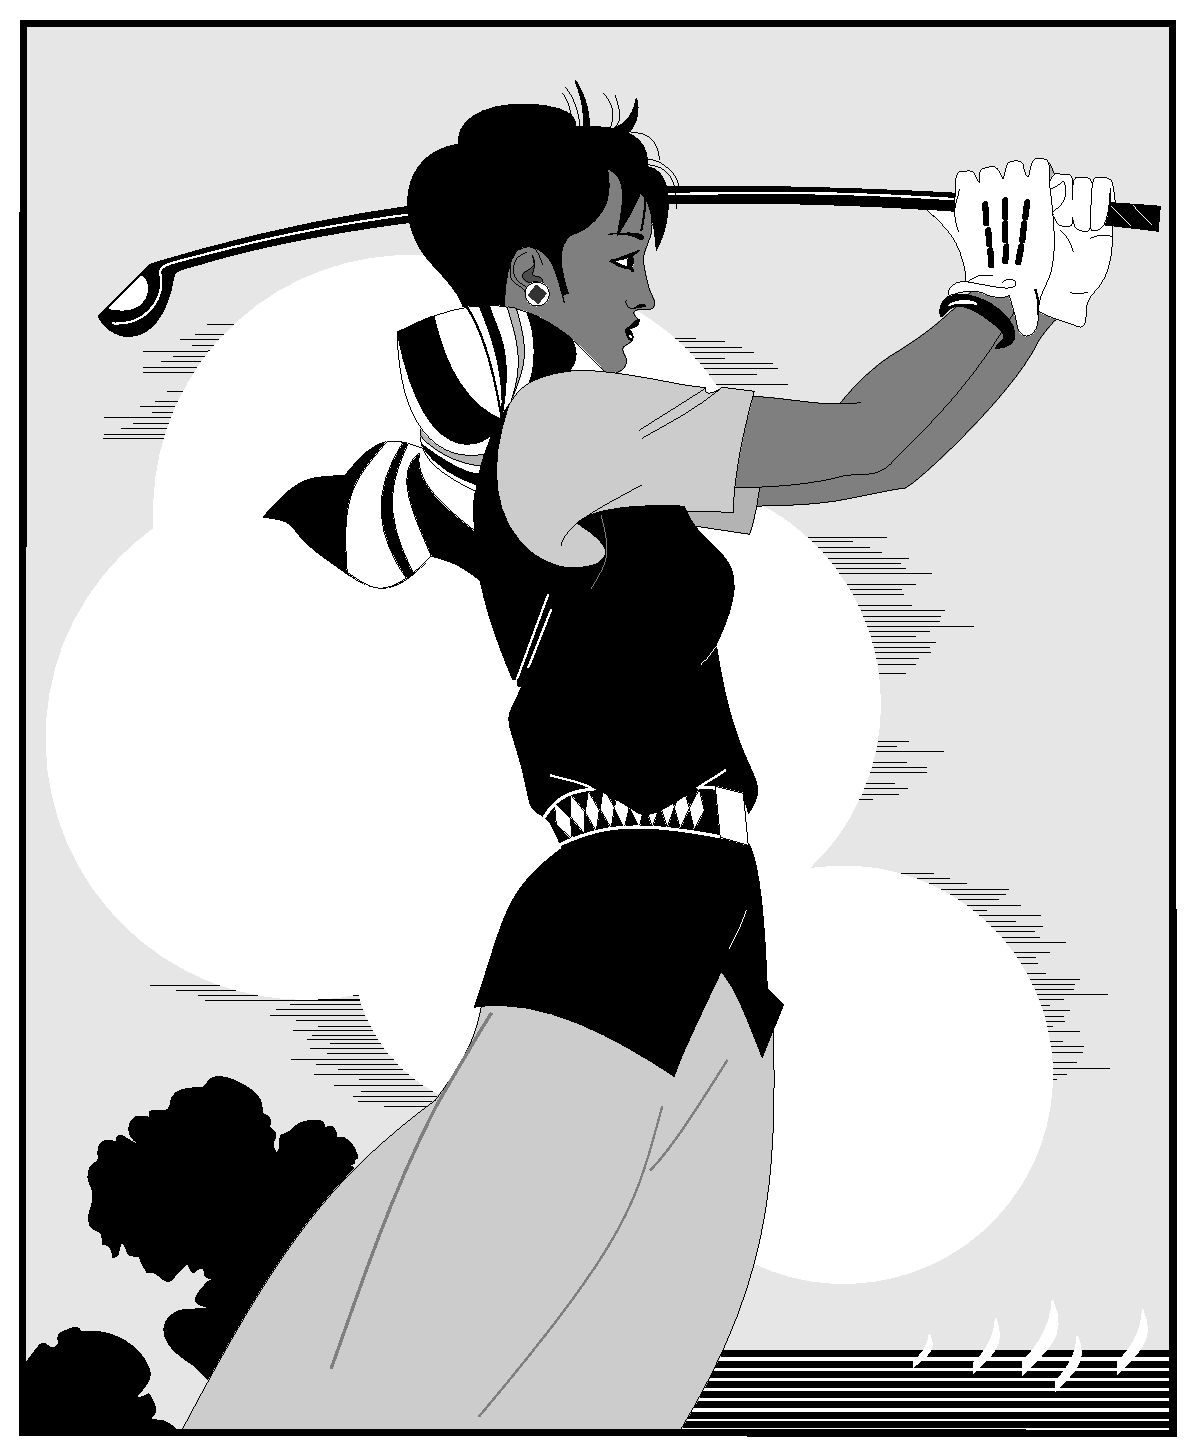
\includegraphics[width = 0.4\textwidth]{golfer}
% \bicaption[golfer1]{}{注意,如果这里字数过长,模板会自动选择最佳字号
% }{Fig.$\!$}{The person playing golf}
% \end{figure}
% \end{latex}
% 单张单图题的格式如下,
% \begin{latex}
% \begin{figure}[h]
% \centering
% 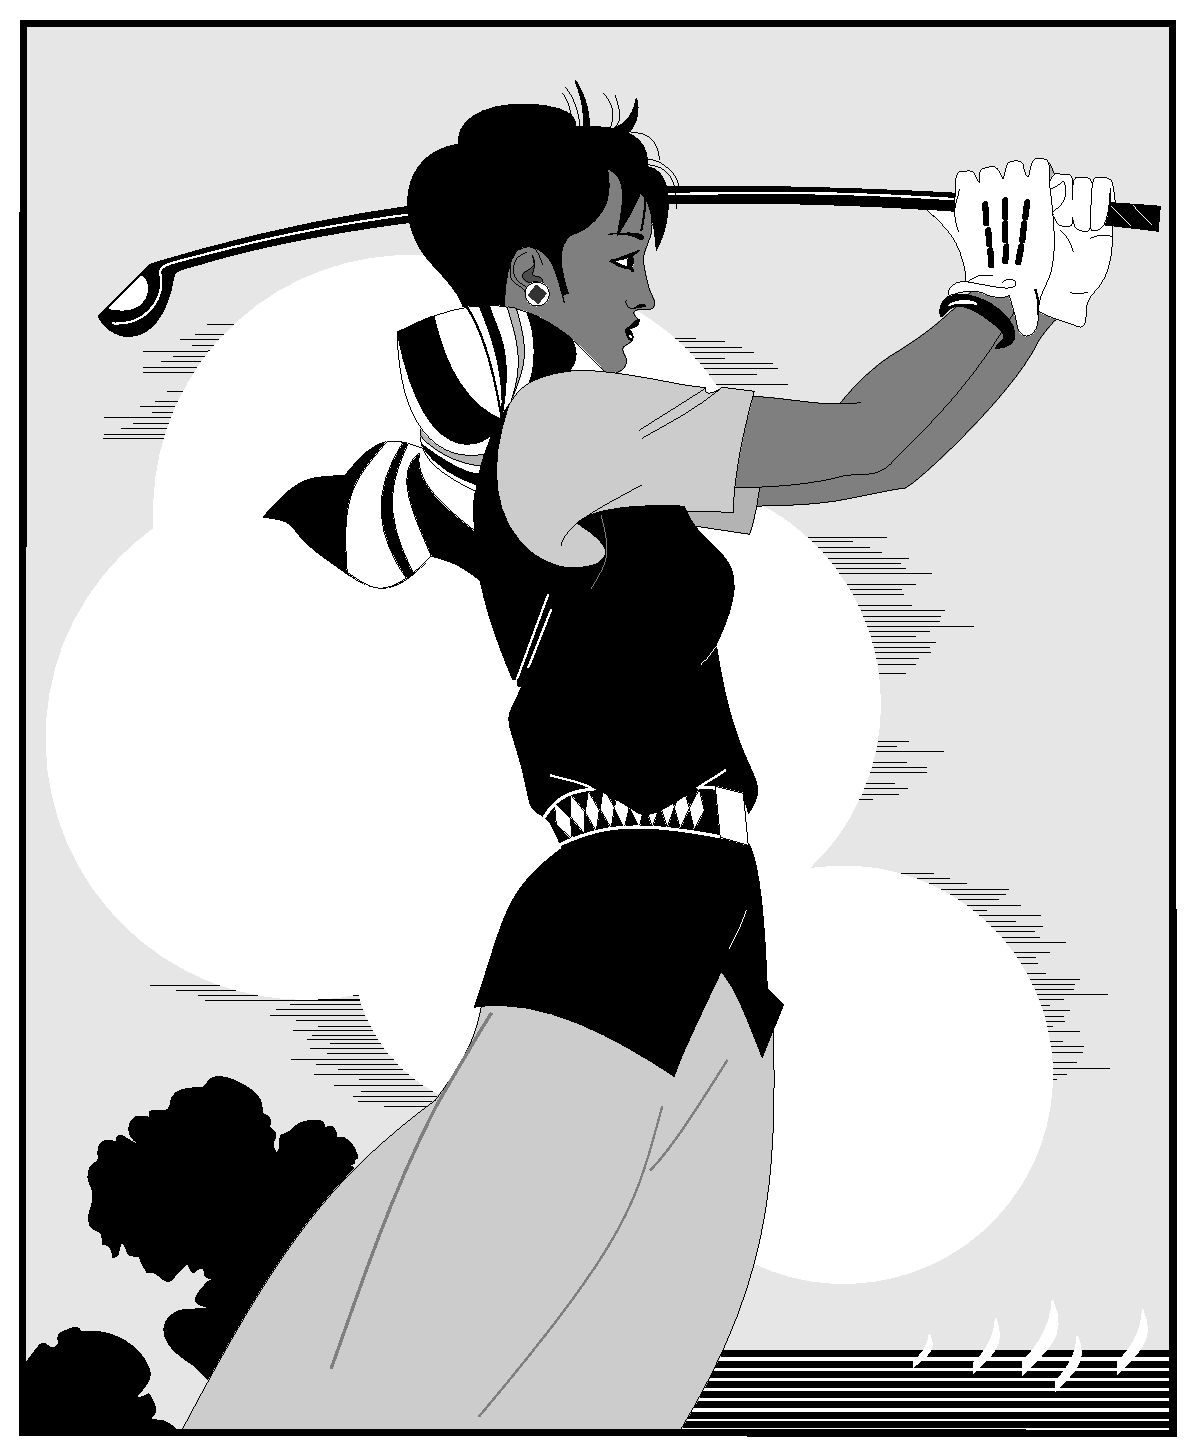
\includegraphics[width = 0.4\textwidth]{golfer}
% \caption{注意,如果这里字数过长,模板会自动选择最佳字号}
% \end{figure}
% \end{latex}
% 带有子图的双语格式,
%
% \subsubsection{公式}
% \subsubsection{数学环境}
% \label{sec:math}
% \hithesis\ 定义了常用的数学环境:
%
% \begin{center}
% \begin{tabular}{*{7}{l}}\toprule
%   axiom & theorem & definition & proposition & lemma & conjecture &\\
%   公理 & 定理 & 定义 & 命题 & 引理 & 猜想 &\\\midrule
%   proof & corollary & example & exercise & assumption & remark & problem \\
%   证明 & 推论 & 例子& 练习 & 假设 & 注释 & 问题\\\bottomrule
% \end{tabular}
% \end{center}
%
% 比如:
% \begin{latex}
% \begin{definition}
%   道千乘之国,敬事而信,节用而爱人,使民以时。
% \end{definition}
% \end{latex}
% 产生(自动编号):
% \medskip
%
% \noindent\framebox[\linewidth][l]{{\heiti 定义~1.1~~~} % {道千乘之国,敬事而信,节用而爱人,使民以时。}}
%
% \smallskip
% 列举出来的数学环境毕竟是有限的,如果想用\emph{胡说}这样的数学环境,那么可以定义:
% \begin{latex}
% \newtheorem{nonsense}{胡说}[chapter]
% \end{latex}
%
% 然后这样使用:
% \begin{latex}
% \begin{nonsense}
%   契丹武士要来中原夺武林秘笈。—— 慕容博
% \end{nonsense}
% \end{latex}
% 产生(自动编号):
%
% \medskip
% \noindent\framebox[\linewidth][l]{{\heiti 胡说~1.1~~~} % {契丹武士要来中原夺武林秘笈。—— 慕容博}}
%
% \subsubsection{算法}
%
% \subsubsection{引用参考文献}
% \DescribeMacro{\inlinecite}
% 学校要求的参考文献引用有两种模式:(1)上标模式。比如``同样的工作有很
% 多$^{[1,2]}$\ldots''。(2)正文模式。比如``文[3] 中详细说明了\ldots''。其中上标
% 模式使用远比正文模式频繁,所以为了符合使用习惯,上标模式仍然用常规
% 的 \cs{cite}\marg{key},而 \cs{inlinecite}\marg{key} 则用来生成正文模式。
%
% 关于参考文献模板推荐使用 \BibTeX,关于中文参考文献需要额外增加一个 Entry:
% \texttt{lang},将其设置为 \texttt{zh} 用来指示此参考文献为中文,以
% 便 \file{hithesis.bst} 处理。如:
% \begin{latex}
% @INPROCEEDINGS{cnproceed,
%   author    = {王重阳 and 黄药师 and 欧阳峰 and 洪七公 and 段皇帝},
%   title     = {武林高手从入门到精通},
%   booktitle = {第~$N$~次华山论剑},
%   year      = 2006,
%   address   = {西安, 中国},
%   month     = sep,
%   lang      = "zh",
% }
%
% @ARTICLE{cnarticle,
%   AUTHOR  = "贾宝玉 and 林黛玉 and 薛宝钗 and 贾探春",
%   TITLE   = "论刘姥姥食量大如牛之现实意义",
%   JOURNAL = "红楼梦杂谈",
%   PAGES   = "260--266",
%   VOLUME  = "224",
%   YEAR    = "1800",
%   LANG    = "zh",
% }
% \end{latex}
%
% 注意如果不需要引用参考文献,请删除 \file{main.tex} 中 \cs{bibliography} 开头的两行,
% 以避免可能的编译错误。
%
% \subsubsection{列表环境}
% \DescribeEnv{itemize}
% \DescribeEnv{enumerate}
% \DescribeEnv{description}
% 为了适合中文习惯,模板将这三个常用的列表环境用 \pkg{enumitem} 进行了纵向间距压
% 缩。一方面清除了多余空间,另一方面用户可以自己指定列表环境的样式(如标签符号,
% 缩进等)。细节请参看 \pkg{enumitem} 文档,此处不再赘述。
% \subsection{后文}
%
% \subsubsection{结论}
% \DescribeEnv{conclusion}
% 结论之后为后文内容。
% \begin{latex}
% \begin{conclusions}
%
% 学位论文的结论作为论文正文的最后一章单独排写,但不加章标题序号。
%
% 结论应是作者在学位论文研究过程中所取得的创新性成果的概要总结,不能与摘要混为一
% 谈。博士学位论文结论应包括论文的主要结果、创新点、展望三部分,在结论中应概括论
% 文的核心观点,明确、客观地指出本研究内容的创新性成果(含新见解、新观点、方法创
% 新、技术创新、理论创新),并指出今后进一步在本研究方向进行研究工作的展望与设想
% 。对所取得的创新性成果应注意从定性和定量两方面给出科学、准确的评价,分(1)、
% (2)、(3)…条列出,宜用“提出了”、“建立了”等词叙述。
%
% \end{conclusions}
% \end{latex}
%
% \subsubsection{参考文献}
% 在后文中的参考文献是自动生成的,不需要用户干预,具体命令在\file{main.tex}中有
% 示例。
%
% \subsubsection{附录}
% \DescribeEnv{appendix}
% 所有的附录都插到这里来。因为附录会更改默认的 chapter 属性,而后面的{\heiti 个人简
%   历}又需要恢复,所以实现为环境可以保证全局的属性不受影响。
% \begin{latex}
% \begin{appendix}
% % -*-coding: utf-8 -*-
%%%%%%%%%%%%%%%%%%%%%%%%%%%%%%%%%%%%%%%%%%%%%%%%%%%%%%%%%
\chapter{带章节的附录}[Full Appendix]%
完整的附录内容,包含章节,公式,图表等

%%%%%%%%%%%%%%%%%%%%%%%%%%%%%%%%%%%%%%%%%%%%%%%%%%%%%%%%%
\section{附录节的内容}[Section in Appendix]
这是附录的节的内容

附录中图的示例:
\begin{figure}[htbp]
\centering
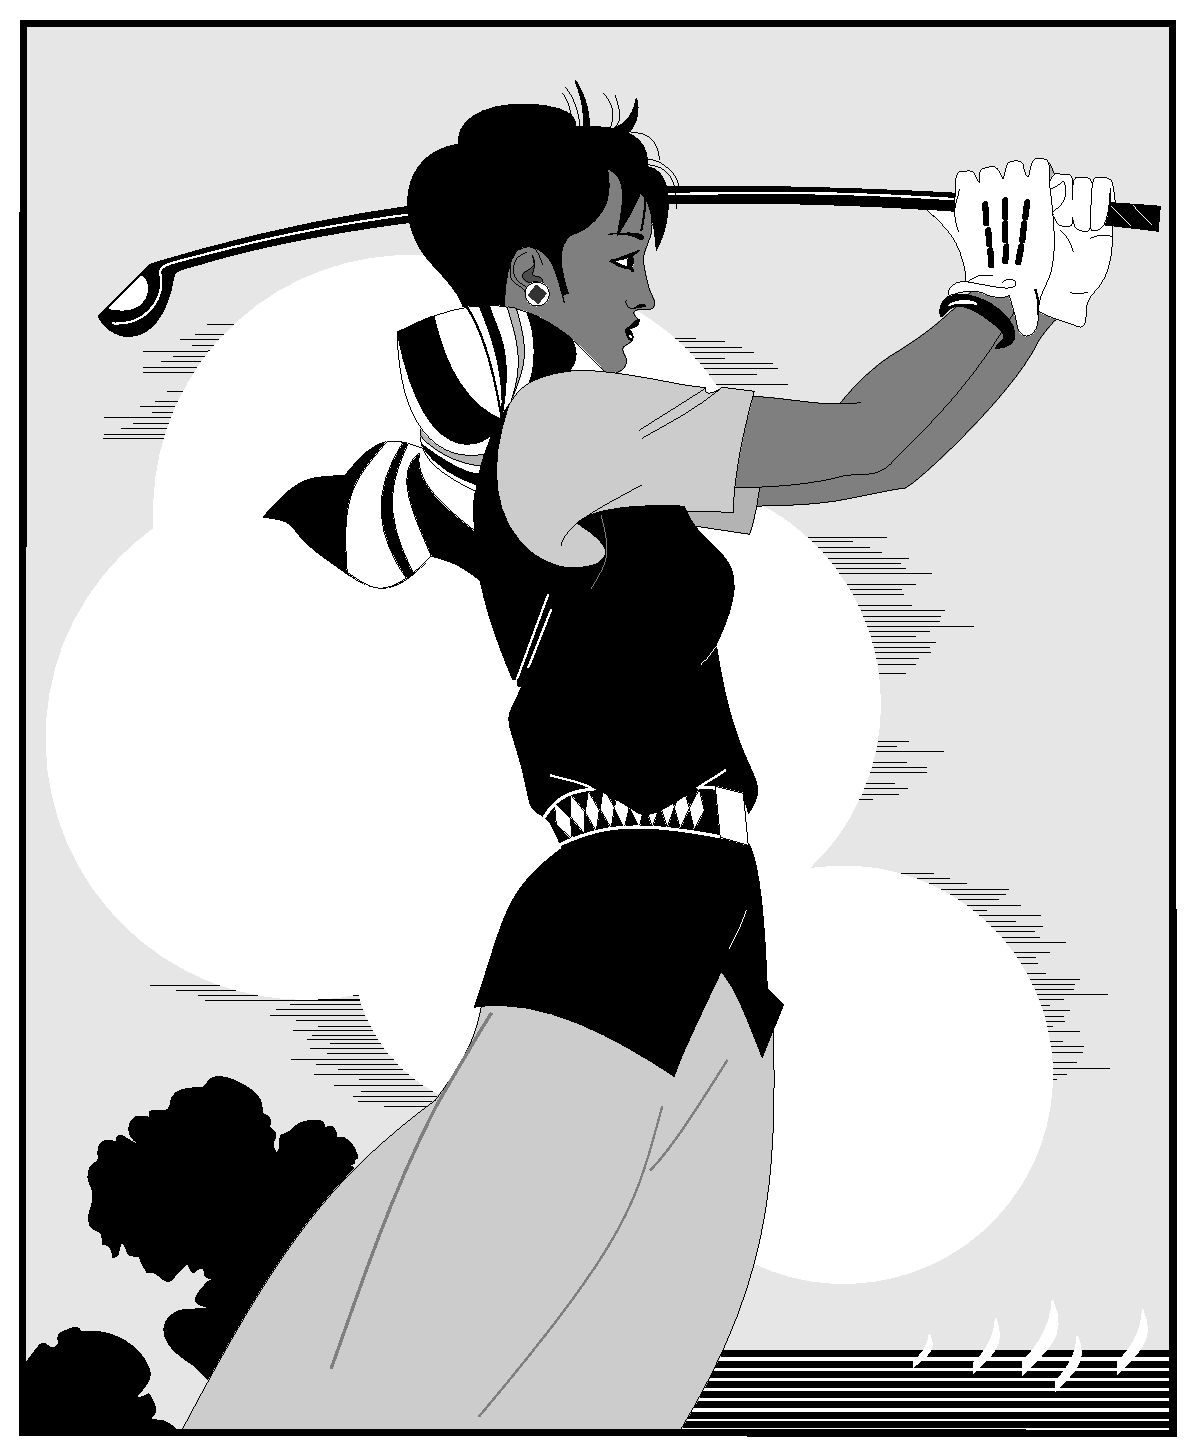
\includegraphics[width = 0.4\textwidth]{golfer}
%\bicaption[golfer5]{}{\xiaosi[0]打高尔夫球的人}{Fig.$\!$}{The person playing golf}\vspace{-1em}
\caption{\xiaosi[0]打高尔夫球的人}
\end{figure}

附录中公式的示例:
\begin{align}
a & = b \times c \\
E & = m c^2
\label{eq}
\end{align}

\chapter{这个星球上最好的免费Linux软件列表}[List of the Best Linux Software in our Planet]
\section*{系统}

\href{http://fvwm.org/}{FVWM 星球最强大的窗口管理器}——推荐

\section*{其他}

\href{https://github.com/goldendict/goldendict}{goldendict 星球最强大的桌面字典}——推荐

\href{http://www.mutt.org/}{mutt 星球最强大的邮件客户端}——推荐

% \end{appendix}
% \end{latex}
%
% \subsubsection{所发表文章}
% \DescribeEnv{publication}
% 虽然在\PGR\UGR\ 中都没有明确规定此处的格式,但按照旧模板PlutoThesis,此处格式
% 非常复杂。此处仍然使用旧模板中的设置方法。
% \begin{latex}
% \begin{publication}
% \noindent\textbf{(一)发表的学术论文}
% \begin{publist}
% \item	XXX,XXX. Static Oxidation Model of Al-Mg/C Dissipation Thermal Protection Materials[J]. Rare Metal Materials and Engineering, 2010, 39(Suppl. 1): 520-524.(SCI~收录,IDS号为~669JS,IF=0.16)
% \item XXX,XXX. 精密超声振动切削单晶铜的计算机仿真研究[J]. 系统仿真学报,2007,19(4):738-741,753.(EI~收录号:20071310514841)
% \item XXX,XXX. 局部多孔质气体静压轴向轴承静态特性的数值求解[J]. 摩擦学学报,2007(1):68-72.(EI~收录号:20071510544816)
% \item XXX,XXX. 硬脆光学晶体材料超精密切削理论研究综述[J]. 机械工程学报,2003,39(8):15-22.(EI~收录号:2004088028875)
% \item XXX,XXX. 基于遗传算法的超精密切削加工表面粗糙度预测模型的参数辨识以及切削参数优化[J]. 机械工程学报,2005,41(11):158-162.(EI~收录号:2006039650087)
% \item XXX,XXX. Discrete Sliding Mode Cintrok with Fuzzy Adaptive Reaching Law on 6-PEES Parallel Robot[C]. Intelligent System Design and Applications, Jinan, 2006: 649-652.(EI~收录号:20073210746529)
% \end{publist}
%
% \noindent\textbf{(二)申请及已获得的专利(无专利时此项不必列出)}
% \begin{publist}
% \item XXX,XXX. 一种温热外敷药制备方案:中国,88105607.3[P]. 1989-07-26.
% \end{publist}
%
% \noindent\textbf{(三)参与的科研项目及获奖情况}
% \begin{publist}
% \item	XXX,XXX. XX~气体静压轴承技术研究, XX~省自然科学基金项目.课题编号:XXXX.
% \item XXX,XXX. XX~静载下预应力混凝土房屋结构设计统一理论. 黑江省科学技术二等奖, 2007.
% \end{publist}
% %\vfill
% %\hangafter=1\hangindent=2em\noindent
% %\setlength{\parindent}{2em}
% \end{publication}
% \end{latex}
%
% \subsubsection{索引}
% \DescribeEnv{ceindex}
% 我工要求中英文双语索引。后文中的自动索引实际上不需要用户干预。
%\begin{latex}
% \begin{ceindex}
%   %如果想要手动加索引,注释掉以下这一样,用wordlist环境
% \printsubindex*
% \end{ceindex}
%\end{latex}
% 手工添加索引的方法不推荐,模板中将去除该功能。
% \subsubsection{授权}
% \DescribeMacro{\authorization}
% 授权页中的签名和日期是需要手写,不需要人工干预。具体示例在\file{main.tex}中。
%\begin{latex}
% \authorization %授权
% %\authorization[saomiao.pdf] %添加扫描页的命令,与上互斥
%\end{latex}
%
% \subsubsection{致谢声明}
% \DescribeEnv{acknowledgement}
% 把致谢做成一个环境更好一些,直接往里面写感谢的话就可以啦!
% \begin{latex}
% \begin{acknowledgement}
%   …
%   感谢\hit\LaTeX\ 论文模板\hithesis\ !
% \end{acknowledgement}
% \end{latex}
%
%
% \subsubsection{简历}
% \DescribeEnv{resume}
% 个人简历。
% 实际上,致谢和个人简历是自由发挥的地区,字体,文体,格式,内容,完全自己决定。
% \begin{latex}
% \begin{resume}
% XXXX~年~XX~月~XX~日出生于~XXXX。
%
% XXXX~年~XX~月考入~XX~大学~XX~院(系)XX~专业,XXXX~年~XX~月本科毕业并获得~XX~学学士学位。
%
% XXXX~年~XX~月------XXXX~年~XX~月在~XX~大学~XX~院(系)XX~学科学习并获得~XX~学硕士学位。
%
% XXXX~年~XX~月------XXXX~年~XX~月在~XX~大学~XX~院(系)XX~学科学习并获得~XX~学博士学位。
%
% 获奖情况:如获三好学生、优秀团干部、X~奖学金等(不含科研学术获奖)。
%
% 工作经历:
% \end{resume}
% \end{latex}
%
% \subsection{其它}
% 模板的配置文件 \file{hithesis.cfg} 中定义了很多固定词汇,一般无须修改。如果有特殊需求,
% 推荐在导言区使用 \cs{renewcommand}。
%
% \StopEventually{\PrintChanges\PrintIndex}
% \clearpage
%
% \section{实现细节}
%
% \subsection{基本信息}
%    \begin{macrocode}
%<cls>\NeedsTeXFormat{LaTeX2e}[1999/12/01]
%<cls>\ProvidesClass{hithesis}
%<cfg>\ProvidesFile{hithesis.cfg}
%<cls|cfg>[2017/08/21 0.0.1 Harbin Institute of Technology]
%    \end{macrocode}
%
% \subsection{定义选项}
% \label{sec:defoption}
%    \begin{macrocode}
%<*cls>
\RequirePackage{ifthen}
\RequirePackage{kvoptions}
\SetupKeyvalOptions{
  family=hit,
  prefix=hit@,
  setkeys=\kvsetkeys}
\newif\ifhit@bachelor
\newif\ifhit@master
\newif\ifhit@doctor
\define@key{hit}{type}{%
  \hit@bachelorfalse
  \hit@masterfalse
  \hit@doctorfalse
  \expandafter\csname hit@#1true\endcsname}
%    \end{macrocode}
% 目录中英文是否用 Arial 字体(默认关闭)。
%    \begin{macrocode}
\DeclareBoolOption[false]{arialtoc}
%    \end{macrocode}
% 章节标题中的英文是否用 Arial 字体(默认打开)。
%    \begin{macrocode}
\DeclareBoolOption[false]{arialtitle}
%    \end{macrocode}
% \option{raggedbottom} 选项(默认关闭)。
%    \begin{macrocode}
\DeclareBoolOption[false]{raggedbottom}
%    \end{macrocode}
% 在脚注标记中使用 \pkg{pifont} 的带圈数字(默认关闭)。
%    \begin{macrocode}
\DeclareBoolOption[false]{pifootnote}
%    \end{macrocode}
% 字体间距设置(默认关闭)。
%    \begin{macrocode}
\DeclareBoolOption[false]{glue}
%    \end{macrocode}
% 文科生四级目录设置(默认关闭)。
%    \begin{macrocode}
\DeclareBoolOption[false]{tocfour}
%    \end{macrocode}
% 目录中“目录”位置是否空行(默认开启)。
%    \begin{macrocode}
\DeclareBoolOption[true]{tocblank}
%    \end{macrocode}
% 章标题是否悬挂居中(默认开启)
%    \begin{macrocode}
\DeclareBoolOption[true]{chapterhang}
%    \end{macrocode}
% 是否是全日制学生(默认是)。
%    \begin{macrocode}
\DeclareBoolOption[true]{fulltime}
%    \end{macrocode}
% 是否有子标题(默认是)。
%    \begin{macrocode}
\DeclareBoolOption[false]{subtitle}
%    \end{macrocode}
% 是否开启debug模式(默认否)。如果开启,载入显示行号等的包,只为开发调试用。
%    \begin{macrocode}
\DeclareBoolOption[false]{debug}
%    \end{macrocode}
% 是否使用新的版心设置(默认否)。
%    \begin{macrocode}
\DeclareBoolOption[false]{newgeometry}
%    \end{macrocode}
% 是否使用右开页(默认否)。
%    \begin{macrocode}
\DeclareBoolOption[false]{openright}
%    \end{macrocode}
% 图题和标题是否居中对其(默认是,非规范要求)。
%    \begin{macrocode}
\DeclareBoolOption[true]{caplastcenter}
%    \end{macrocode}
% 声明字体选项。
%    \begin{macrocode}
\DeclareStringOption{fontset}
%    \end{macrocode}
% 将其余选项默认传递给 \pkg{ctexbook}。
%    \begin{macrocode}
\DeclareDefaultOption{\PassOptionsToClass{\CurrentOption}{ctexbook}}
%    \end{macrocode}
% 解析用户传递过来的选项,并加载 \pkg{ctexbook}。
%    \begin{macrocode}
\ProcessKeyvalOptions*
%    \end{macrocode}
% 使用 \XeTeX\ 引擎时,\pkg{fontspec} 宏包会被 \pkg{xeCJK} 自动调用。传递
% 给 \pkg{fontspec} 宏包 \option{no-math} 选项,避免部分数学符号字体自动调整
% 为 CMR。其他引擎下没有这个问题,这一行会被无视。
%    \begin{macrocode}
\PassOptionsToPackage{no-math}{fontspec}
%    \end{macrocode}
% 载入单双面打印设置,本、硕单面,博士双面。
%    \begin{macrocode}
\ifhit@bachelor
\PassOptionsToClass{oneside}{book}
\fi
\ifhit@master
\PassOptionsToClass{oneside}{book}
\fi
\ifhit@doctor
\PassOptionsToClass{twoside}{book}
\fi
%    \end{macrocode}
% 设置字体。由于宋体没有粗体,且我工模板的标题要求使用粗宋体,于是面临CTeX的经典
% 的伪粗体bug:“首次出现伪粗体字体之后的正常字体无法复制”。但如果使用自带宋体的
% 思源字体,那么不必使用伪粗体。
%    \begin{macrocode}
\ifthenelse%
{\equal{\hit@fontset}{}}%
{%
  \PassOptionsToPackage{AutoFakeBold=2}{xeCJK}
}%
{%
  \ifthenelse%
  {\equal{\hit@fontset}{siyuan}}%
  {\relax}%
  {%
    \PassOptionsToPackage{AutoFakeBold=2}{xeCJK}
  }%
  \PassOptionsToClass{fontset=\hit@fontset}{ctexbook}
}%
%    \end{macrocode}
% 使用 \pkg{ctexbook} 类,优于调用 \pkg{ctex} 宏包。
%    \begin{macrocode}
\LoadClass[a4paper,openany,UTF8,zihao=-4,scheme=plain]{ctexbook}
%    \end{macrocode}
% 用户至少要提供一个选项,指定论文类型。
%    \begin{macrocode}
\ifhit@bachelor\relax\else
  \ifhit@master\relax\else
    \ifhit@doctor\relax\else
        \ClassError{hithesis}%
                   {Please specify thesis type in option: \MessageBreak
                    type=[bachelor | master | doctor]}{}
      \fi
  \fi
\fi
%    \end{macrocode}
%
% \subsection{装载宏包}
% \label{sec:loadpackage}
%
% 引用的宏包和相应的定义。
%    \begin{macrocode}
\RequirePackage{etoolbox}
\RequirePackage{ifxetex}
\ifxetex
\else
        \ClassError{hithesis}%
                   {Please use: \MessageBreak
                    xelatex}{}
\fi
\RequirePackage{xparse}
%    \end{macrocode}
%
% \AmSTeX\ 宏包,用来排出更加漂亮的公式。
%    \begin{macrocode}
\RequirePackage{amsmath}
%    \end{macrocode}
%
% \pkg{newtx} 设置 Times New Roman,Helvetica。
%    \begin{macrocode}
\RequirePackage[defaultsups]{newtxtext}
\RequirePackage{newtxmath}
%    \end{macrocode}
% \pkg{newtx} 的 Mono 字体虽然很好看,但在论文中不常见。学校虽未要求 Mono 字体,
% 还是选择常见的 Courier 字体。由于比较新的实现 \TeX\ Gyre Cursor 会修
% 改\cs{bfdefault},导致中文加粗出问题,所以选用标准 \pkg{courier}。
%    \begin{macrocode}
\RequirePackage{courier}
%    \end{macrocode}
% 图形支持宏包。
%    \begin{macrocode}
\RequirePackage{graphicx}
%    \end{macrocode}
% \pkg{pdfpages} 宏包便于我们插入扫描后的授权页和声明页 PDF 文档。
%    \begin{macrocode}
\RequirePackage{pdfpages}
\includepdfset{fitpaper=true}
%    \end{macrocode}
% 更好的列表环境。
%    \begin{macrocode}
\RequirePackage{enumitem}       %使用enumitem宏包,改变列表项的格式
\RequirePackage{environ}
%    \end{macrocode}
% 禁止 \LaTeX 自动调整多余的页面底部空白,并保持脚注仍然在底部。
% 脚注按页编号。
%    \begin{macrocode}
\ifhit@raggedbottom
  \RequirePackage[bottom,perpage,hang]{footmisc}
  \raggedbottom
\else
  \RequirePackage[perpage,hang]{footmisc}
\fi
%    \end{macrocode}
% 脚注格式。
%    \begin{macrocode}
\ifhit@pifootnote
  \RequirePackage{pifont}
\fi
%    \end{macrocode}
% 利用 \pkg{CJKfntef} 实现汉字的下划线和盒子内两段对齐,并可以避免
% \cs{makebox}\oarg{width}\oarg{s} 可能产生的 underful boxes。
%    \begin{macrocode}
\RequirePackage{CJKfntef}
%    \end{macrocode}
% 定理类环境宏包,其中 \pkg{amsmath} 选项用来兼容 \AmSTeX\ 的宏包
%    \begin{macrocode}
\RequirePackage[amsmath,thmmarks,hyperref]{ntheorem}
%    \end{macrocode}
% 表格控制
%    \begin{macrocode}
\RequirePackage{longtable}
%    \end{macrocode}
% 使用三线表:\cs{toprule},\cs{midrule},\cs{bottomrule}。
%    \begin{macrocode}
\RequirePackage{booktabs}
%    \end{macrocode}
% 参考文献引用宏包。
%    \begin{macrocode}
\RequirePackage[sort&compress]{natbib}
%    \end{macrocode}
% 生成有书签的 pdf 及其开关,请结合 gbk2uni 避免书签乱码。
%    \begin{macrocode}
\RequirePackage{hyperref}
\hypersetup{%
  CJKbookmarks=true,
  linktoc=all,
  bookmarksnumbered=true,
  bookmarksopen=true,
  bookmarksopenlevel=1,
  breaklinks=true,
  colorlinks=false,
  plainpages=false,
  pdfborder=0 0 0}
%    \end{macrocode}
% 设置 url 样式,与上下文一致
%    \begin{macrocode}
\urlstyle{same}
%    \end{macrocode}
%
% \subsection{页面设置}
% \label{sec:layout}
% 本来这部分应该是最容易设置的,但根据我工\PGR\ 的3.8,3.4,3.2节的版芯矛盾,此处
% 设置两种版芯。
%    \begin{macrocode}
\ifhit@debug\RequirePackage[showframe]{geometry}\else\RequirePackage{geometry}\fi
\geometry{%根据PlutoThesis 原版定义而来
  a4paper, % 210 * 297mm
  hcentering,
  ignoreall,
  nomarginpar,
}
\ifhit@newgeometry%
\geometry{
  centering,
  text={150true mm,240true mm},
  left=30true mm,
  head=5true mm,
  headsep=0true mm,
  footskip=0true mm,
  foot=0true mm
}
\else%
\geometry{%根据PlutoThesis 原版定义而来
  text={150true mm,224true mm},
  top=35.5true mm,
  left=30true mm,
  head=5true mm,
  headsep=2.5true mm,
  foot=8.5true mm
}
\fi
%    \end{macrocode}
%    载入显示行号的包。
%    \begin{macrocode}
\ifhit@debug%
\RequirePackage{layout}
\RequirePackage{lineno}
\fi
%    \end{macrocode}
% 利用 \pkg{fancyhdr} 设置页眉页脚。
%    \begin{macrocode}
\RequirePackage{fancyhdr}
%    \end{macrocode}
% 其他包,表格、彩色、数学符号包
%    \begin{macrocode}
\RequirePackage{tabularx}
\RequirePackage{varwidth}
\RequirePackage{multicol}
\RequirePackage{color}          % 支持彩色
\RequirePackage{amssymb}
\RequirePackage[below]{placeins}%允许上一个section的浮动图形出现在下一个section的开始部分,还提供\FloatBarrier命令,使所有未处理的浮动图形立即被处理
\RequirePackage{flafter}       % 使得所有浮动体不能被放置在其浮动环境之前,以免浮动体在引述它的文本之前出现.
\RequirePackage{multirow}       %使用Multirow宏包,使得表格可以合并多个row格
\RequirePackage[hang]{subfigure}%支持子图 %centerlast 设置最后一行是否居中
\RequirePackage[subfigure]{ccaption} %支持双语标题
%    \end{macrocode}
%    中英文索引包。
%    \begin{macrocode}
\RequirePackage[makeindex]{splitidx}
\newindex[]{china}
\newindex[]{english}
%</cls>
%    \end{macrocode}
%    我工要求的索引格式。
%    \begin{macrocode}
%<*ist>
headings_flag 1
heading_prefix "\{\\centering\\normalsize\\textbf\{"
heading_suffix "\}\\par\}\\nopagebreak\\wuhao\n"
delim_0 "\\hspace{2em}"
delim_1 "\\hspace{2em}"
%</ist>
%    \end{macrocode}
%    算法。
%    \begin{macrocode}
%<*cls>
\RequirePackage[boxed,linesnumbered,algochapter]{algorithm2e}  % 算法的宏包,注意宏包兼容性,先后顺序为float、hyperref、algorithm(2e),否则无法生成算法列表
%    \end{macrocode}
%    logo。
%    \begin{macrocode}
\RequirePackage{xltxtra}
\def\hithesis{\textsc{hi}\-\textsc{Thesis}}
%    \end{macrocode}
%    排版源码。
%    \begin{macrocode}
\RequirePackage{listings}
\lstset{
%basicstyle=\small\ttfamily,
columns=flexible,
breaklines=true
}
%</cls>
%    \end{macrocode}
%
% \subsection{主文档格式}
% \label{sec:mainbody}
%
% \subsubsection{Three matters}
% \begin{macro}{\cleardoublepage}
% 对于 \textsl{openright} 选项,必须保证章首页右开,且如果前章末页无内容须
% 清空其页眉页脚。
%    \begin{macrocode}
%<*cls>
\let\hit@cleardoublepage\cleardoublepage
\newcommand{\hit@clearemptydoublepage}{%
  \clearpage{\pagestyle{hit@empty}\hit@cleardoublepage}
}
\let\cleardoublepage\hit@clearemptydoublepage
%    \end{macrocode}
% \end{macro}
% \begin{macro}{\frontmatter}
% \begin{macro}{\mainmatter}
% \begin{macro}{\backmatter}
% 我们的单面和双面模式与常规的不太一样。
%    \begin{macrocode}
\renewcommand\frontmatter{%
  \ifhit@openright\cleardoublepage\else\clearpage\fi
  \@mainmatterfalse
  \pagenumbering{Roman}
  \pagestyle{hit@empty}
}

\renewcommand\mainmatter{%
  \ifhit@tocblank%
  \addtocontents{toc}{\vspace{\baselineskip}} %规范中并没有这一要求,此处不应该加
  \addtocontents{toe}{\vspace{\baselineskip}}
  \fi%
  \ifhit@openright\cleardoublepage\else\clearpage\fi
  \@mainmattertrue
  \pagenumbering{arabic}
  \pagestyle{hit@headings}
}

\renewcommand\backmatter{%
  \ifhit@openright\cleardoublepage\else\clearpage\fi
  \@mainmattertrue}
%</cls>
%    \end{macrocode}
% \end{macro}
% \end{macro}
% \end{macro}
%
% \subsubsection{字体}
% \label{sec:font}
% \begin{macro}{\normalsize}
% 根据我工规定,正文小四号 (12bp) 字,行距为固定值3--4mm。
%    \begin{macrocode}
%<*cls>
\renewcommand\normalsize{%
  \@setfontsize\normalsize{12bp}{\ifhit@glue 20.50398bp \@plus 2.83465bp \@minus 0bp\else 20.50398bp\fi}%
  \abovedisplayskip=8pt
  \abovedisplayshortskip=8pt
  \belowdisplayskip=\abovedisplayskip
  \belowdisplayshortskip=\abovedisplayshortskip}
%    \end{macrocode}
% \end{macro}
%
% WORD 中的字号对应该关系如下(1bp = 72.27/72 pt):
% \begin{center}
% \begin{tabular}{llll}
% \toprule
% 初号 & 42bp & 14.82mm & 42.1575pt \\
% 小初 & 36bp & 12.70mm & 36.135 pt \\
% 一号 & 26bp & 9.17mm & 26.0975pt \\
% 小一 & 24bp & 8.47mm & 24.09pt \\
% 二号 & 22bp & 7.76mm & 22.0825pt \\
% 小二 & 18bp & 6.35mm & 18.0675pt \\
% 三号 & 16bp & 5.64mm & 16.06pt \\
% 小三 & 15bp & 5.29mm & 15.05625pt \\
% 四号 & 14bp & 4.94mm & 14.0525pt \\
% 小四 & 12bp & 4.23mm & 12.045pt \\
% 五号 & 10.5bp & 3.70mm & 10.59375pt \\
% 小五 & 9bp & 3.18mm & 9.03375pt \\
% 六号 & 7.5bp & 2.56mm & \\
% 小六 & 6.5bp & 2.29mm & \\
% 七号 & 5.5bp & 1.94mm & \\
% 八号 & 5bp & 1.76mm & \\\bottomrule
% \end{tabular}
% \end{center}
%
% \begin{macro}{\hit@def@fontsize}
% 根据习惯定义字号。用法:\cs{hit@def@fontsize}\marg{字号名称}\marg{磅数}避免了
% 字号选择和行距的紧耦合。所有字号定义时为单倍行距,并提供选项指定行距倍数。
%    \begin{macrocode}
\def\hit@def@fontsize#1#2{%
  \expandafter\newcommand\csname #1\endcsname[1][1.3]{%
    \fontsize{#2}{##1\dimexpr #2}\selectfont}}
%    \end{macrocode}
% \end{macro}
%
% \begin{macro}{\chuhao}
% \begin{macro}{\xiaochu}
% \begin{macro}{\yihao}
% \begin{macro}{\xiaoyi}
% \begin{macro}{\erhao}
% \begin{macro}{\xiaoer}
% \begin{macro}{\sanhao}
% \begin{macro}{\xiaosan}
% \begin{macro}{\sihao}
% \begin{macro}{\banxiaosi}
% \begin{macro}{\xiaosi}
% \begin{macro}{\dawu}
% \begin{macro}{\wuhao}
% \begin{macro}{\xiaowu}
% \begin{macro}{\liuhao}
% \begin{macro}{\xiaoliu}
% \begin{macro}{\qihao}
% \begin{macro}{\bahao}
% 一组字号定义。
%    \begin{macrocode}
\hit@def@fontsize{chuhao}{42bp}
\hit@def@fontsize{xiaochu}{36bp}
\hit@def@fontsize{yihao}{26bp}
\hit@def@fontsize{xiaoyi}{24bp}
\hit@def@fontsize{erhao}{22bp}
\hit@def@fontsize{xiaoer}{18bp}
\hit@def@fontsize{sanhao}{16bp}
\hit@def@fontsize{xiaosan}{15bp}
\hit@def@fontsize{sihao}{14bp}
\hit@def@fontsize{banxiaosi}{13bp}
\hit@def@fontsize{xiaosi}{12bp}
\hit@def@fontsize{dawu}{11bp}
\hit@def@fontsize{wuhao}{10.5bp}
\hit@def@fontsize{xiaowu}{9bp}
\hit@def@fontsize{liuhao}{7.5bp}
\hit@def@fontsize{xiaoliu}{6.5bp}
\hit@def@fontsize{qihao}{5.5bp}
\hit@def@fontsize{bahao}{5bp}
%</cls>
%    \end{macrocode}
% \end{macro}
% \end{macro}
% \end{macro}
% \end{macro}
% \end{macro}
% \end{macro}
% \end{macro}
% \end{macro}
% \end{macro}
% \end{macro}
% \end{macro}
% \end{macro}
% \end{macro}
% \end{macro}
% \end{macro}
% \end{macro}
% \end{macro}
% \end{macro}
% \subsubsection{页眉页脚}
% \label{sec:headerfooter}
% \begin{macro}{\hit@empty}
% \begin{macro}{\hit@plain}
% \begin{macro}{\hit@headings}
% 定义三种页眉页脚格式:
% \begin{itemize}
% \item \texttt{hit@empty}:页眉页脚都没有
% \item \texttt{hit@plain}:只显示页脚的页码。\cs{chapter} 自动调用
% \cs{thispagestyle\{hit@plain\}}。
% \item \texttt{hit@headings}:页眉页脚同时显示
% \end{itemize}
%    \begin{macrocode}
%<*cls>
\let\hit@headrule\headrule
\fancypagestyle{hit@empty}{%
  \fancyhf{}
  \let\headrule\hit@headrule%
  \renewcommand{\headrulewidth}{0pt}
  \renewcommand{\footrulewidth}{0pt}
}

\fancypagestyle{hit@plain}{%
  \fancyhead{}
  \fancyfoot[C]{\xiaowu\thepage}
  \renewcommand{\headrulewidth}{0pt}
  \renewcommand{\footrulewidth}{0pt}
}

\fancypagestyle{hit@headings}{%
  \fancyhf{}
  \ifhit@doctor
  \fancyhead[CO]{\songti\xiaowu[0]\leftmark}
  \fancyhead[CE]{\songti\xiaowu[0]\hit@cschoolname\hit@cdegree\hit@cthesisname}%
  \else
  \ifhit@master
  \fancyhead[C]{\songti\xiaowu[0]\hit@cschoolname\hit@cdegree\hit@cthesisname}
  \fi
  \fi
  \ifhit@bachelor
  \fancyhead[C]{\songti\xiaowu[0]\hit@cschoolname\hit@bachelor@cxuewei\hit@bachelor@cthesisname}%
  \fancyfoot[C]{\xiaowu \thepage}
  \else
  \fancyfoot[C]{\xiaowu -~\thepage~-}
  \fi
  % 此处可能和word模板不一致
  % 页眉中小五汉字,0行距时,占用9bt,页眉高度为14pt, 所以以下数字之和要保持等于14pt-9bt=4.96634pt
  % 根据PlutoThesis模板中rule宽度定义为2.25, 0.75, 保持粗线和细线之间的间距为细线宽度。
  % 如果页眉是多行的情况,rule向下溢出
  \renewcommand{\headrule}{
    \vskip 1.190132pt
    \hrule\@height2.276208pt\@width\headwidth
    \vskip 0.75pt
    \hrule\@height.75pt\@width\headwidth
  }
  \renewcommand{\footrulewidth}{0pt}
}

\AtBeginDocument{%此处解决页眉经典bug
  \pagestyle{hit@empty}
  \renewcommand{\chaptermark}[1]{\@mkboth{\CTEXthechapter\enspace#1}{}}}
%</cls>
%    \end{macrocode}
% \end{macro}
% \end{macro}
% \end{macro}
%
%
% \subsubsection{段落}
% \label{sec:paragraph}
%
% 全文首行缩进 2 字符,标点符号用全角
%    \begin{macrocode}
%<*cls>
\ctexset{%
  punct=quanjiao,
  space=auto,
  autoindent=true}
%    \end{macrocode}
% 利用 \pkg{enumitem} 命令调整默认列表环境间的距离,以符合中文习惯。
%    \begin{macrocode}
\setlist{nosep}
%</cls>
%    \end{macrocode}
% \subsubsection{脚注}
% \label{sec:footnote}
% 脚注符合中文习惯,数字带圈。
%    \begin{macrocode}
%<*cls>
\def\hit@textcircled#1{%
  \ifnum\value{#1} >9
    \ClassError{hithesis}%
      {Too many footnotes in this page.}{Keep footnote less than 10.}
  \fi
  \ifhit@pifootnote%
    \ding{\the\numexpr\value{#1}+171\relax}%
  \else%
    \textcircled{\xiaoliu\arabic{#1}}%
  \fi}
\renewcommand{\thefootnote}{\hit@textcircled{footnote}}
\renewcommand{\thempfootnote}{\hit@textcircled{mpfootnote}}
%    \end{macrocode}
% 定义脚注分割线,字号(宋体小五),以及悬挂缩进(1.5字符)。
%    \begin{macrocode}
\def\footnoterule{\vskip-3\p@\hrule\@width0.3\textwidth\@height0.4\p@\vskip2.6\p@}
\let\hit@footnotesize\footnotesize
\renewcommand\footnotesize{\hit@footnotesize\xiaowu[1.5]}
\footnotemargin1.5em\relax
%    \end{macrocode}
% \cs{@makefnmark} 默认是上标样式,而在脚注部分要求为正文大小。利用\cs{patchcmd}
% 动态调整 \cs{@makefnmark} 的定义。
%    \begin{macrocode}
\let\hit@makefnmark\@makefnmark
\def\hit@@makefnmark{\hbox{{\normalfont\@thefnmark}}}
\pretocmd{\@makefntext}{\let\@makefnmark\hit@@makefnmark}{}{}
\apptocmd{\@makefntext}{\let\@makefnmark\hit@makefnmark}{}{}
%</cls>
%    \end{macrocode}
% \subsubsection{数学相关}
% \label{sec:equation}
% 允许太长的公式断行、分页等。
%    \begin{macrocode}
%<*cls>
\allowdisplaybreaks[4]
\predisplaypenalty=0  %公式之前可以换页,公式出现在页面顶部
\renewcommand\theequation{\ifnum \c@chapter>\z@ \thechapter-\fi\@arabic\c@equation}
%    \end{macrocode}
% 公式距前后文的距离由 4 个参数控制,参见 \cs{normalsize} 的定义。
% 同时为了让 \pkg{amsmath} 的 \cs{tag*} 命令得到正确的格式,我们必须修改这些代
% 码。\cs{make@df@tag} 是定义 \cs{tag*} 和 \cs{tag} 内部命令的。
% \cs{make@df@tag@@} 处理 \cs{tag*},我们就改它!
% \begin{latex}
% \def\make@df@tag{\@ifstar\make@df@tag@@\make@df@tag@@@}
% \def\make@df@tag@@#1{%
%   \gdef\df@tag{\maketag@@@{#1}\def\@currentlabel{#1}}}
% \end{latex}
%    \begin{macrocode}
\def\make@df@tag{\@ifstar\hit@make@df@tag@@\make@df@tag@@@}
\def\hit@make@df@tag@@#1{\gdef\df@tag{\hit@maketag{#1}\def\@currentlabel{#1}}}
\iffalse
\ifhit@bachelor
  \def\hit@maketag#1{\maketag@@@{%
    (\ignorespaces\text{\equationname\hskip0.5em}#1\unskip\@@italiccorr)}}
  \def\tagform@#1{\maketag@@@{%
    (\ignorespaces\text{\equationname\hskip0.5em}#1\unskip\@@italiccorr)\equcaption{#1}}}
\fi
\fi
\def\hit@maketag#1{\maketag@@@{(\ignorespaces #1\unskip\@@italiccorr)}}
\def\tagform@#1{\maketag@@@{(\ignorespaces #1\unskip\@@italiccorr)\equcaption{#1}}}
%    \end{macrocode}
% 修改 \cs{tagform} 会影响 \cs{eqref}。
%    \begin{macrocode}
\renewcommand{\eqref}[1]{\textup{(\ref{#1})}}
%</cls>
%    \end{macrocode}
% 定理标题使用黑体,正文使用宋体,冒号隔开。
%    \begin{macrocode}
%<*cfg>
\theorembodyfont{\normalfont}
\theoremheaderfont{\normalfont\heiti}
\theoremsymbol{\ensuremath{\square}}
\newtheorem*{proof}{证明}
\theoremstyle{plain}
\theoremsymbol{}
\theoremseparator{:}
\newtheorem{assumption}{假设}[chapter]
\newtheorem{definition}{定义}[chapter]
\newtheorem{proposition}{命题}[chapter]
\newtheorem{lemma}{引理}[chapter]
\newtheorem{theorem}{定理}[chapter]
\newtheorem{axiom}{公理}[chapter]
\newtheorem{corollary}{推论}[chapter]
\newtheorem{exercise}{练习}[chapter]
\newtheorem{example}{例}[chapter]
\newtheorem{remark}{注释}[chapter]
\newtheorem{problem}{问题}[chapter]
\newtheorem{conjecture}{猜想}[chapter]
%</cfg>
%    \end{macrocode}
% \subsubsection{浮动对象以及表格}
% \label{sec:float}
% 设置浮动对象和文字之间的距离
%    \begin{macrocode}
%<*cls>
\setlength{\floatsep}{\ifhit@glue 20.50398bp \@plus 2.83465bp \@minus 0bp\else 21bp\fi}
\setlength{\intextsep}{\ifhit@glue 20.50398bp \@plus 2.83465bp \@minus 0bp\else 21bp\fi}
\setlength{\textfloatsep}{\ifhit@glue 20.50398bp \@plus 2.83465bp \@minus 0bp\else 21bp\fi}
\setlength{\@fptop}{0bp}
\setlength{\@fpsep}{12bp}
\setlength{\@fpbot}{0bp}
%    \end{macrocode}
% 下面这组命令使浮动对象的缺省值稍微宽松一点,从而防止幅度对象占据过多的文本页面,
% 也可以防止在很大空白的浮动页上放置很小的图形。
%    \begin{macrocode}
\renewcommand{\textfraction}{0.15}
\renewcommand{\topfraction}{0.85}
\renewcommand{\bottomfraction}{0.65}
\renewcommand{\floatpagefraction}{0.60}
%    \end{macrocode}
% 由于我工的双标题,导致标题之下多出一空白字符的距离,去除。
%    \begin{macrocode}
\let\hit@oldfigure\figure
\let\hit@oldendfigure\endfigure
\def\figure{\begingroup\hit@oldfigure}
\def\endfigure{\vskip-1em\hit@oldendfigure\endgroup}
\let\hit@oldtable\table
\let\hit@oldendtable\endtable
\def\table{\begingroup\hit@oldtable}
\def\endtable{\vskip-1em\hit@oldendtable\endgroup}
%    \end{macrocode}
% 我工要求,标题字数多使用小五字体,否则使用五号字体。
% 此处定义过多为超过两行。
%    \begin{macrocode}
\newlength{\hit@captionlength}
\long\def\@makecaption#1#2{%
  \settowidth{\hit@captionlength}{#2}
  \ifhit@bachelor\wuhao[1.667]\else\ifdim\hit@captionlength>300mm\xiaowu[1.667]\else\wuhao[1.667]\fi\fi
  \vskip\abovecaptionskip
  \ifhit@caplastcenter\centering\fi\sbox\@tempboxa{#1\ifhit@bachelor\hskip\ccwd\else\enskip\fi#2}%
  \ifdim \wd\@tempboxa >\hsize
  #1\ifhit@bachelor\hskip\ccwd\else\enskip\fi#2\par
  \else
  \global \@minipagefalse
  \hb@xt@\hsize{\hfil\box\@tempboxa\hfil}%
  \fi
\vskip\belowcaptionskip}
%    \end{macrocode}
% 我们采用 \pkg{longtable} 来处理跨页的表格。同样我们需要设置其默认字体为五号。
%    \begin{macrocode}
\let\hit@LT@array\LT@array
\def\LT@array{\dawu[1.5]\hit@LT@array} % set default font size
%    \end{macrocode}
%    图表算法名称及格式。TODO:修改
%    \begin{macrocode}
\renewcommand{\thesubtable}{(\alph{subtable})}
\renewcommand{\thefigure}{\arabic{chapter}-\arabic{figure}}%使图编号为 7-1 的格式 %\protect{~}
\renewcommand{\thesubfigure}{\alph{subfigure})}%使子图编号为 a)的格式
\renewcommand{\p@subfigure}{\thefigure~} %使子图引用为 7-1 a) 的格式,母图编号和子图编号之间用~加一个空格
\renewcommand{\thetable}{\arabic{chapter}-\arabic{table}}%使表编号为 7-1 的格式
\renewcommand{\theequation}{\arabic{chapter}-\arabic{equation}}%使公式编号为 7-1 的格式
\newcommand{\algoenname}{Algo.} %算法英文标题
\newfloatlist[chapter]{algoen}{aen}{\listalgoenname}{\algoenname}
\newfixedcaption{\algoencaption}{algoen}
\renewcommand{\thealgoen}{\thechapter-\arabic{algocf}}
\renewcommand{\@cftmakeaentitle}{\chapter*{\listalgoenname\@mkboth{\bfseries\listalgoenname}{\bfseries\listalgoenname}}
}
\renewcommand{\algorithmcfname}{算法}
\setlength\AlCapSkip{1.2ex}
\SetAlgoSkip{1pt}
\renewcommand{\algocf@captiontext}[2]{\wuhao#1\algocf@typo ~ \AlCapFnt{}#2} % text of caption
\expandafter\ifx\csname algocf@within\endcsname\relax% if \algocf@within doesn't exist
\renewcommand\thealgocf{\@arabic\c@algocf} % and the way it is printed
\else%                                    else
\renewcommand\thealgocf{\csname the\algocf@within\endcsname-\@arabic\c@algocf}
\fi
\renewcommand{\algocf@makecaption}[2]{%中英文双标题一定多于一行,因此去掉单行时的判断,并将\parbox中标题设置为居中
  \addtolength{\hsize}{\algomargin}%
  \sbox\@tempboxa{\algocf@captiontext{#1}{#2}}%
    \hskip .5\algomargin%
    \parbox[t]{\hsize}{\centering\algocf@captiontext{#1}{#2}}%
  \addtolength{\hsize}{-\algomargin}%
}
\newcommand{\AlgoBiCaption}[2]{%直接取出自定义的中英文标题条目加入到真正的\caption 中
   \caption[#1]{\protect\setlength{\baselineskip}{1.5em}#1 \protect \\ Algo. \thealgocf~~ #2} % \algoencaption{#2}
   \addcontentsline{aen}{algoen}{\protect\numberline{\thealgoen}{#2}}
}
%    \end{macrocode}
%    调整罗列环境、浮动格式、间距。
%    \begin{macrocode}
% 调整罗列环境的布局
\setitemize{leftmargin=0em,itemsep=0em,partopsep=0em,parsep=0em,topsep=0em,itemindent=3em}
\setenumerate{leftmargin=0em,itemsep=0em,partopsep=0em,parsep=0em,topsep=0em,itemindent=3.5em}
\newcommand{\citeup}[1]{\textsuperscript{\cite{#1}}}
% 定制浮动图形和表格标题样式
\captionnamefont{\wuhao[1.667]}
\captiontitlefont{\wuhao[1.667]}
\captiondelim{~~}
\hangcaption
\renewcommand{\subcapsize}{\wuhao[1.667]}
\setlength{\abovecaptionskip}{0pt}%为了双标题之间的间距,不能设置
\setlength{\belowcaptionskip}{0pt}
% 自定义项目列表标签及格式 \begin{publist} 列表项 \end{publist}
\newcounter{pubctr} %自定义新计数器
\newenvironment{publist}{%%%%%定义新环境
\begin{list}{[\arabic{pubctr}]} %%标签格式
    {
     \usecounter{pubctr}
     \setlength{\leftmargin}{1.7em}     % 左边界 \leftmargin =\itemindent + \labelwidth + \labelsep
     \setlength{\itemindent}{0em}     % 标号缩进量
     \setlength{\labelsep}{0.5em}       % 标号和列表项之间的距离,默认0.5em
     \setlength{\rightmargin}{0em}    % 右边界
     \setlength{\topsep}{0ex}         % 列表到上下文的垂直距离
     \setlength{\parsep}{0ex}         % 段落间距
     \setlength{\itemsep}{0ex}        % 标签间距
     \setlength{\listparindent}{0pt} % 段落缩进量
    }}
{\end{list}}
% 设置定理定义格式
\theoremstyle{plain}
\theorembodyfont{\songti\rmfamily}
\theoremheaderfont{\heiti\rmfamily}
\theoremsymbol{$\square$}
\setlength{\theorempreskipamount}{0pt}
\setlength{\theorempostskipamount}{-2pt}
\setlength{\parindent}{2em}
\arraycolsep=1.6pt
%</cls>
%    \end{macrocode}
%
% \subsubsection{章节标题}
% \label{sec:theor}
%    \begin{macrocode}
%<*cfg>
\ctexset{%
  chapter/name={第,章},
  appendixname=附录,
  contentsname={目\hspace{\ccwd}录},
  listfigurename=插图索引,
  listtablename=表格索引,
  figurename=图,
  tablename=表,
  bibname=参考文献,
  indexname=索引,
}
\newcommand\listfigureename{Index of figure}
\newcommand\listtableename{Index of table}
\newcommand\listequationename{Index of equation}
\newcommand\listequationname{公式索引}
\newcommand\equationname{公式}
\newcommand{\cabstractcname}{摘\hspace{\ccwd}要}
\newcommand{\cabstractename}{Abstract (In Chinese)}
\newcommand{\eabstractcname}{Abstract}
\def\hit@doctor@eabstract@ename{ABSTRACT}
\newcommand{\eabstractename}{Abstract (In English)}
\newcommand{\hit@ckeywords@title}{关键词:}
\def\hit@ckeywords@separator{;}
\def\hit@ekeywords@separator{,}
\let\CJK@todaysave=\today
\def\CJK@todaysmall@short{\the\year 年 \the\month 月}
\def\CJK@todaysmall{\the\year 年 \the\month 月 \the\day 日}
\def\CJK@todaybig@short{\zhdigits{\the\year}年\zhnumber{\the\month}月}
\def\CJK@todaybig{\zhdigits{\the\year}年\zhnumber{\the\month}月\zhnumber{\the\day}日}
\def\CJK@today{\CJK@todaysmall}
\renewcommand\today{\CJK@today}
\newcommand\CJKtoday[1][1]{%
  \ifcase#1\def\CJK@today{\CJK@todaysave}
    \or\def\CJK@today{\CJK@todaysmall}
    \or\def\CJK@today{\CJK@todaybig}
  \fi}
\cdate{\ifhit@bachelor\CJK@todaysmall\else\CJK@todaybig@short\fi}
\edate{\ifcase \month \or January\or February\or March\or April\or May%
       \or June\or July \or August\or September\or October\or November
       \or December\fi\unskip,\ \ \the\year}
%</cfg>
%    \end{macrocode}
% 按照我工要求,页面中标题之下不少于一行。
%    \begin{macrocode}
%<*cls>
\def\hit@title@font{%
  \ifhit@arialtitle\sffamily\else\heiti\fi}

\newcommand\hit@chapter@titleformat[1]{%开启悬挂缩进选项
    \ifthenelse%
      {\equal{#1}{\eabstractcname}}%
      {\bfseries #1}%
      %实现章标题的居中加悬挂缩进,注意,此处一定是\CTEX@chaptername\CTEX@chapter@aftername, 否则是英文标题长度
      {\ifhit@chapterhang\settowidth{\hangindent}{\CTEX@chaptername\CTEX@chapter@aftername}\hangafter=1\fi#1}%
      %{\begin{varwidth}[t]{\hit@chapter@indentboxwidth}#1\end{varwidth}}
}

\renewcommand\@afterheading{%
  \@nobreaktrue
  \everypar{%
    \if@nobreak
      \@nobreakfalse
      \clubpenalty 1
      \if@afterindent \else
        {\setbox\z@\lastbox}%
      \fi
    \else
      \clubpenalty 1
      \everypar{}%
    \fi}}
%    \end{macrocode}
% 设置一到四级标题、目录、书签格式。
%    \begin{macrocode}
\ctexset{%
  chapter={
    afterindent=true,
    pagestyle={hit@headings},
    beforeskip={28.34658bp},%一个空行 1.57481 × 18
    afterskip={24.74658bp},%0.8应该不计算间距 0.8 × 18 + 0.57481×18
    aftername=\enspace,
    format={\centering\hit@title@font\xiaoer[1.57481]},%\center 会影响之后全局
    nameformat=\relax,
    numberformat=\relax,
    titleformat=\hit@chapter@titleformat,
    fixskip=true, % 添加这一行去除默认间距
    %hang=true,
  },
  section={
    afterindent=true,
    beforeskip={\ifhit@glue 13.5bp \@plus 1.677267bp \@minus 1.157391bp \else 13.5bp \fi},%上下空0.5行
    afterskip={\ifhit@glue 13.5bp \@plus 1.677267bp \@minus 1.157391bp  \else 13.5bp \fi},
    format={\hit@title@font\ifhit@glue\fontsize{15bp}{21bp \@plus 1.677267bp \@minus 1.157391bp}\else\fontsize{15bp}{21bp}\fi\selectfont},
    aftername=\enspace,
    fixskip=true,
    break={},
  },
  subsection={
    afterindent=true,
    beforeskip={\ifhit@glue 11bp \@plus 1.842609bp \@minus 0.9920497bp \else 11bp \fi},
    afterskip={\ifhit@glue 11bp \@plus 2.33863bp \@minus 0.49602bp \else 11bp \fi},
    format={\hit@title@font\ifhit@glue\fontsize{14bp}{18bp \@plus 1.842609bp \@minus 0.9920497bp}\else\fontsize{14bp}{18bp}\fi\selectfont},
    aftername=\enspace,
    fixskip=true,
    break={},
  },
  subsubsection={
    afterindent=true,
    beforeskip={\ifhit@glue 8.50398bp \@plus 2.83465bp \@minus 0bp \else 9bp \fi},
    afterskip={\ifhit@glue 8.50398bp \@plus 2.83465bp \@minus 0bp \else 9bp \fi},
    format={\hit@title@font\normalsize},
    aftername=\enspace,
    fixskip=true,
    break={},
  },
  paragraph/afterindent=true,
  subparagraph/afterindent=true
}
%    \end{macrocode}
%    设置附表、附录格式。
%    \begin{macrocode}
\NewDocumentCommand{\hit@appendix@chapter}{s m o}{%
  \IfBooleanT{#1}%
  {
    \phantomsection
    \markboth{#2}{#2}
    \addcontentsline{toc}{chapter}{\ifhit@arialtitle\sffamily\heiti\else\heiti\fi #2}
    \IfValueT{#3}{\addcontentsline{toe}{chapter}{\bfseries #3}}
    \hit@chapter*{#2}
  }
}
% 该附录命令适用于发表文章,简历等
\newcommand{\BiAppChapter}[2]    % 该附录命令适用于有章节的完整附录
{\phantomsection
 \chapter{#1}
 \addcontentsline{toe}{chapter}{\bfseries \xiaosi Appendix \thechapter~~#2}
}
%    \end{macrocode}
%    设置章节命令。s: 星号,表示在目录中出不出现序号。m: 必须要有的选项,中文章
%    节名称也即目录中名称,页眉中名称,书签中的名称。o: 可选内容,没有就默认是正
%    文章节,如果有,则是英文目录中显示的内容。
%    \begin{macro}{\chapter}
%    \begin{macro}{\section}
%    \begin{macro}{\subsection}
%    \begin{macro}{\subsubsection}
%    \begin{macrocode}
\let\hit@chapter\chapter
\RenewDocumentCommand{\chapter}{s o m o}{%
  \ifhit@openright\cleardoublepage\else\clearpage\fi\phantomsection%
  \IfBooleanTF{#1}%
  {%	if \chapter*
    \hit@chapter*{#3}%
    \IfValueT{#4}{%
      \addcontentsline{toe}{chapter}{\bfseries #4}
    }
  }%
  {%	if \chapter
    \IfNoValueTF{#2}%
    {\hit@chapter{#3}}%
    {\hit@chapter[#2]{#3}}%
    \IfValueT{#4}{%
    \addcontentsline{toe}{chapter}{\bfseries\relax Chapter \thechapter\hspace{0.5em} #4}
    }
  }
}

\let\hit@section\section
\RenewDocumentCommand\section{s o m o}{
  \IfBooleanTF{#1}%
  {%	if \section*
    \hit@section*{#3}%
    \IfValueT{#4}{%
      \addcontentsline{toe}{section}{#4}
    }
  }%
  {%	if \section
    \IfNoValueTF{#2}%
    {\hit@section{#3}}%
    {\hit@section[#2]{#3}}%
    \IfValueT{#4}{%
    \addcontentsline{toe}{section}{\protect\numberline{\csname thesection\endcsname} #4}
    }
  }
}

\let\hit@subsection\subsection
\RenewDocumentCommand\subsection{s o m o}{
  \IfBooleanTF{#1}%
  {%	if \subsection*
    \hit@subsection*{#3}%
    \IfValueT{#4}{%
      \addcontentsline{toe}{subsection}{#4}
    }
  }%
  {%	if \subsection
    \IfNoValueTF{#2}%
    {\hit@subsection{#3}}%
    {\hit@subsection[#2]{#3}}%
    \IfValueT{#4}{%
    \addcontentsline{toe}{subsection}{\protect\numberline{\csname thesubsection\endcsname} #4}
    }
  }
}

\let\hit@subsubsection\subsubsection
\RenewDocumentCommand\subsubsection{s o m o}{
  \IfBooleanTF{#1}%
  {%	if \subsubsection*
    \hit@subsubsection*{#3}%
    \IfValueT{#4}{%
      \addcontentsline{toe}{subsubsection}{#4}
    }
  }%
  {%	if \subsubsection
    \IfNoValueTF{#2}%
    {\hit@subsubsection{#3}}%
    {\hit@subsubsection[#2]{#3}}%
    \IfValueT{#4}{%
    \addcontentsline{toe}{subsubsection}{\protect\numberline{\csname thesubsubsection\endcsname} #4}
    }
  }
}
%    \end{macrocode}
%    \end{macro}
%    \end{macro}
%    \end{macro}
%    \end{macro}
%
% \subsubsection{定义封面}
% \label{sec:cov}
% 封面信息。
%    \begin{macrocode}
\def\hit@def@term#1{%
  \define@key{hit}{#1}{\csname #1\endcsname{##1}}
  \expandafter\gdef\csname #1\endcsname##1{%
    \expandafter\gdef\csname hit@#1\endcsname{##1}}
  \csname #1\endcsname{}}

\hit@def@term{statesecrets} %密级
\hit@def@term{natclassifiedindex}  %国内图书分类号
\hit@def@term{internatclassifiedindex}  %国际图书分类号

\hit@def@term{ctitle} %中文标题
\hit@def@term{csubtitle} %中文副标题
\hit@def@term{cxueke} %中文学科
\hit@def@term{cauthor} %中文作者
\hit@def@term{csupervisor} %中文导师
\hit@def@term{cassosupervisor} %中文副导师
\hit@def@term{ccosupervisor}%中文联合导师
\hit@def@term{caffil}%中文院系
\hit@def@term{csubject}%中文专业
\hit@def@term{cdate}

\hit@def@term{cstudentid}%
\hit@def@term{cstudenttype}%
\hit@def@term{ctitleone}%
\hit@def@term{ctitletwo}%


\hit@def@term{etitle} %英文标题
\hit@def@term{esubtitle} %英文标题
\hit@def@term{exueke} %英文学科
\hit@def@term{eauthor} %英文作者
\hit@def@term{esupervisor} %英文导师
\hit@def@term{eassosupervisor} %英文副导师
\hit@def@term{ecosupervisor} %英文联合导师
\hit@def@term{eaffil}
\hit@def@term{esubject}
\hit@def@term{edate}
\hit@def@term{estudenttype}
\newcommand{\hit@@cabstract}[1]{\long\gdef\hit@cabstract{#1}}
\newenvironment{cabstract}{\Collect@Body\hit@@cabstract}{}
\newcommand{\hit@@eabstract}[1]{\long\gdef\hit@eabstract{#1}}
\newenvironment{eabstract}{\Collect@Body\hit@@eabstract}{}
\def\hit@parse@keywords#1{
  \define@key{hit}{#1}{\csname #1\endcsname{##1}}
  \expandafter\gdef\csname hit@#1\endcsname{}
  \expandafter\gdef\csname #1\endcsname##1{
    \@for\reserved@a:=##1\do{
      \expandafter\ifx\csname hit@#1\endcsname\@empty\else
        \expandafter\g@addto@macro\csname hit@#1\endcsname{%
          \ignorespaces\csname hit@#1@separator\endcsname}
      \fi
      \expandafter\expandafter\expandafter\g@addto@macro%
        \expandafter\csname hit@#1\expandafter\endcsname\expandafter{\reserved@a}}}}
\hit@parse@keywords{ckeywords}
\hit@parse@keywords{ekeywords}
\def\hitsetup{\kvsetkeys{hit}}
%</cls>
%    \end{macrocode}
%   定义封面中用到的词汇。
%    \begin{macrocode}
%<*cfg>
\ifhit@doctor
\gdef\hit@cxueweishort{博}
\gdef\hit@exuewei{Doctor}
\gdef\hit@exueweier{Doctoral}
\gdef\hit@cxuewei{\hit@cxueweishort 士}
\gdef\hit@cdegree{\hit@cxueke\hit@cxuewei}
\gdef\hit@edegree{\hit@exuewei \ of \hit@exueke}
\def\hit@cauthortitle{\hit@cxueweishort 士研究生}
\fi
\ifhit@master
\gdef\hit@cxueweishort{硕}
\gdef\hit@exuewei{Master}
\gdef\hit@exueweier{Master's}
\gdef\hit@cxuewei{\hit@cxueweishort 士}
\gdef\hit@cdegree{\hit@cxueke\hit@cxuewei}
\gdef\hit@edegree{\hit@exuewei \ of \hit@exueke}
\def\hit@cauthortitle{\hit@cxueweishort 士研究生}
\fi
\ifhit@bachelor
\gdef\hit@cxuewei{学士}
\fi
\def\hit@bachelor@cxuewei{本科}
\def\hit@bachelor@cthesisname{毕业设计(论文)}
\def\hit@bachelor@caffiltitle{院(系)}
\def\hit@bachelor@cstudentidtitle{学号}
\def\hit@bachelor@cmajortitle{专业}
\def\hit@bachelor@csupervisortitle{指导教师}
\def\hit@bachelor@cthesistitle{题目}
\def\hit@bachelor@cstudenttitle{学生}
\def\hit@cthesisname{学位论文}
\def\hit@cschoolname{哈尔滨工业大学}
\def\hit@cschoolnametitle{授予学位单位}
\def\hit@cdatetitle{答辩日期}
\def\hit@caffiltitle{所在单位}
\def\hit@csubjecttitle{学科}
\def\hit@cdegreetitle{申请学位}
\def\hit@csupervisortitle{导师}
\def\hit@cassosupervisortitle{副导师}
\def\hit@ccosupervisortitle{联合导师}
\def\hit@title@csep{:}
\def\hit@eauthortitle{Candidate}
\def\hit@esupervisortitle{Supervisor}
\def\hit@eassosupervisortitle{Associate Supervisor}
\def\hit@ecosupervisortitle{Co Supervisor}
\def\hit@edegreetitle{Academic Degree Applied for}
\def\hit@esubjecttitle{Specialty}
\def\hit@eaffiltitle{Affiliation}
\def\hit@edatetitle{Date of Defence}
\def\hit@eschoolnametitle{Degree-Conferring-Institution}
\def\hit@eschoolname{Harbin Institute of Technology}
\def\hit@title@esep{:}
\def\hit@natclassifiedindextitle{国内图书分类号}
\def\hit@internatclassifiedindextitle{国际图书分类号}
\def\hit@secretlevel{密级}
\def\hit@schoolidtitle{学校代码}
\def\hit@schoolid{10213}
\def\hit@conclusion@ctitle{结\hspace{\ccwd}论}
\def\hit@conclusion@etitle{Conclusions}
\def\hit@bibname@etitle{References}
\def\hit@acknowledgement@ctitle{致\hspace{\ccwd}谢}
\def\hit@acknowledgement@etitle{Acknowledgements}
\def\hit@resume@ctitle{个人简历}
\def\hit@resume@etitle{Resume}
\def\hit@authorization@ctitle{哈尔滨工业大学学位论文原创性声明和使用权限}
\def\hit@authorization@etitle{Statement of copyright and Letter of authorization}
\newcommand{\hit@authorsig}{作者签名:}
\newcommand{\hit@teachersig}{导师签名:}
\newcommand{\hit@frontdate}{日期:}
\newcommand{\hit@denotation@ctitle}{物理量名称及符号表}
\newcommand{\hit@denotation@etitle}{List of physical quantity and symbol}
\newcommand{\hit@authorizationtitle}{学位论文使用权限}
\newcommand{\hit@authorizationtext}{%
学位论文是研究生在哈尔滨工业大学攻读学位期间完成的成果,知识产权归属哈尔滨工业大学。学位论文的使用权限如下:

(1)学校可以采用影印、缩印或其他复制手段保存研究生上交的学位论文,并向国家图书馆报送学位论文;(2)学校可以将学位论文部分或全部内容编入有关数据库进行检索和提供相应阅览服务;(3)研究生毕业后发表与此学位论文研究成果相关的学术论文和其他成果时,应征得导师同意,且第一署名单位为哈尔滨工业大学。

保密论文在保密期内遵守有关保密规定,解密后适用于此使用权限规定。

本人知悉学位论文的使用权限,并将遵守有关规定。}
\newcommand{\hit@declarename@bachelor}{哈尔滨工业大学本科毕业设计(论文)原创性声明}
\newcommand{\hit@authorizationtext@bachelor}{%
本人郑重声明:在哈尔滨工业大学攻读学士学位期间,所提交的毕业设计(论文)《\hit@ctitle》,是本人在导师指导下独立进行研究工作所取得的成果。对本文的研究工作做出重要贡献的个人和集体,均已在文中以明确方式注明,其它未注明部分不包含他人已发表或撰写过的研究成果,不存在购买、由他人代写、剽窃和伪造数据等作假行为。

本人愿为此声明承担法律责任。}
\newcommand{\hit@declarename}{学位论文原创性声明}
\newcommand{\hit@declaretext}{%
本人郑重声明:此处所提交的学位论文《\hit@ctitle》,是本人在导师指导下,在哈尔滨工业大学攻读学位期间独立进行研究工作所取得的成果,且学位论文中除已标注引用文献的部分外不包含他人完成或已发表的研究成果。对本学位论文的研究工作做出重要贡献的个人和集体,均已在文中以明确方式注明。}
\newcommand{\hit@datefill}{\hspace{2.5em}年\hspace{1.5em}月\hspace{1.5em}日}
\newcommand{\hit@publication@ctitle}{攻读\hit@cxuewei 学位期间发表的论文及其他成果}
\newcommand{\hit@publication@etitle}{Papers published in the period of PH.D. education}
\def\hit@index@etitle{Index}
\def\hit@hi{嗨!thesis}
\def\hit@cbraceleft{(}
\def\hit@cbraceright{)}
\def\hit@ebraceleft{(}
\def\hit@ebraceright{)}
\newcommand{\pozhehao}{——}
\def\hit{哈尔滨工业大学}
\def\PGR{\href{http://hitgs.hit.edu.cn/aa/fd/c3425a109309/page.htm}
{《\hit 研究生学位论文撰写规范》}}
\def\UGR{\href{http://jwc.hit.edu.cn/2566/list.htm}
{《\hit 本科生毕业论文撰写规范》}}
%</cfg>
%    \end{macrocode}
% 中英文封面。
%    \begin{macrocode}
%<*cls>
\newlength{\hit@title@width}
\newcommand{\hit@put@title}[2][\hit@title@width]{%
  \begin{CJKfilltwosides}[b]{#1}#2\end{CJKfilltwosides}}

\def\hit@first@titlepage{%
  \ifhit@bachelor\hit@first@titlepage@bachelor\else\hit@first@titlepage@other\fi}
\def\hit@second@titlepage{%
  \ifhit@bachelor\hit@second@titlepage@bachelor\else\hit@second@titlepage@other\fi}

\newcommand{\hit@first@titlepage@bachelor}{
\ifthenelse%
{\equal{\hit@fontset}{siyuan}}%
{\xiaosi[1]\vspace*{0.65em}}%
{\xiaosi[1]\textcolor[rgb]{1,1,1}{\songti{\hit@hi}}}%
  \vspace*{1.2cm}
  \begin{center}
    \parbox[t][3.4cm][t]{\textwidth}{
  \begin{center}\erhao[0]\heiti\hit@ctitle\end{center} }
    \parbox[t][9cm][t]{\textwidth}{
    \begin{center}\xiaoer[0]\songti\textbf{\hit@cauthor}\end{center}
  }
  \begin{center}
    \setlength{\hit@title@width}{4em}
    \heiti\xiaosi
      \begin{tabular}{rc}
	{\hit@put@title{\hit@bachelor@caffiltitle}\hit@title@csep} & \hit@caffil\\[14pt]
	{\hit@put@title{\hit@bachelor@cstudentidtitle}\hit@title@csep} & \hit@cstudentid
    \end{tabular}
      \begin{tabular}{rc}
	{\hit@put@title{\hit@bachelor@cmajortitle}\hit@title@csep} & \hit@csubject\\[14pt]
	{\hit@put@title{\hit@bachelor@csupervisortitle}\hit@title@csep} &  \hit@csupervisor
      \end{tabular}
    \end{center}
    \vspace{2.6cm}
    {\xiaosi[0]\songti\textbf{\hit@cdate}}
  \end{center}
}
\newcommand{\hit@second@titlepage@bachelor}{
  \vspace*{0.6cm}
  \centering
\includegraphics[scale=0.38]{logo.pdf}
  \vspace{1.5cm}
  \begin{center}
    \centering
\includegraphics[scale=0.25]{bthesistitle.pdf}
    \vfill
    \parbox[t][14.2cm][b]{\textwidth}
    {\heiti\xiaosan
      \begin{center} \renewcommand{\arraystretch}{2.5} \heiti
	\setlength{\hit@title@width}{5.5em}
	\begin{tabular}{l@{\ \  }c}

	  {\xiaoer  \hit@put@title{\hit@bachelor@cthesistitle}} & \underline{\makebox[6.1cm]{\xiaoer \hit@ctitleone}}\\
								     &  \underline{\makebox[6.1cm]{\xiaoer \hit@ctitletwo}}\\
									    & \\
	  {\hit@put@title{\hit@bachelor@cmajortitle}}                  & \underline{\makebox[6.1cm]{\hit@csubject}}\\
	  {\hit@put@title{\hit@bachelor@cstudentidtitle}}                  & \underline{\makebox[6.1cm]{\hit@cstudentid}}\\
	  {\hit@put@title{\hit@bachelor@cstudenttitle}}                  & \underline{\makebox[6.1cm]{\hit@cauthor}}\\
	  {\hit@put@title{\hit@bachelor@csupervisortitle}} & \underline{\makebox[6.1cm]{\hit@csupervisor}}\\
	  {\hit@put@title{\hit@cdatetitle}} & \underline{\makebox[6.1cm]{\hit@cdate}}
	\end{tabular} \renewcommand{\arraystretch}{1}
      \end{center}
    }
  \end{center}
}

\newlength{\hit@etitlelength}%
\newcommand{\hit@first@titlepage@other}{
  % 封面一
\ifthenelse%
{\equal{\hit@fontset}{siyuan}}%
{\xiaosi[1]\vspace*{0.65em}}%
{\xiaosi[1]\textcolor[rgb]{1,1,1}{\songti{\hit@hi}}}%
 \vspace*{1.2cm}
\begin{center}
  \begin{center}\xiaoyi[1]\songti\textbf{\hit@cxuewei\hit@cthesisname}\end{center}
    \ifhit@fulltime\vspace{1.4cm}\else%
      \begin{center}\xiaoyi[1]\songti\textbf{\hit@cbraceleft\hit@cstudenttype\hit@cbraceright}\end{center}
    \fi%
    \parbox[t][2.8cm][t]{\textwidth}{%
  \begin{center}\erhao\heiti\hit@ctitle\end{center}
\ifhit@subtitle\begin{center}\hspace{-4em}\xiaoer\heiti\pozhehao\hit@csubtitle\end{center}\fi}
    \parbox[t][5.1cm][t]{\textwidth}{%英文标题太长时可以采用\xiaoer
  \begin{center}%
    \settowidth{\hit@etitlelength}{\erhao\hit@etitle\ifhit@subtitle\hit@title@esep\hit@esubtitle\fi}%
    \ifdim\hit@etitlelength>450mm\xiaoer\else\erhao\fi%
    \textbf{\MakeUppercase{\hit@etitle}%
\ifhit@subtitle\hit@title@esep\MakeUppercase{\hit@esubtitle}\fi}\end{center}}
    \parbox[t][7.4cm][t]{\textwidth}{
  \begin{center}\xiaoer\songti\textbf{\hit@cauthor}\end{center}}
    \parbox[t][1.4cm][t]{\textwidth}{
  \begin{center}\kaishu\xiaoer\textbf{\hit@cschoolname}\end{center}}
    {\songti\xiaoer\textbf{\hit@cdate}}
\end{center}
}

%内封
\newcommand{\hit@second@titlepage@other}{
  \begin{center}
    {\songti \xiaosi
      \begin{tabular}{@{}r@{:}l@{}}
	\hit@natclassifiedindextitle & \hit@natclassifiedindex\\
	\hit@internatclassifiedindextitle & \hit@internatclassifiedindex
    \end{tabular}}\hfill
    {\songti \xiaosi
      \begin{tabular}{@{}r@{:}l@{}}
	\hit@schoolidtitle & \hit@schoolid\\
	\hit@secretlevel & \hit@statesecrets
    \end{tabular}}
  \parbox[t][3.2cm][t]{\textwidth}{\begin{center} \end{center} }
    \parbox[t][2.4cm][t]{\textwidth}{\xiaoer[1]
  \begin{center}\songti\bfseries\hit@cdegree\hit@cthesisname\end{center}
      \ifhit@fulltime\relax\else\begin{center}\songti\textbf{\hit@cbraceleft\hit@cstudenttype\hit@cbraceright}\end{center}\fi}
	\parbox[t][5cm][t]{\textwidth}{\erhao
  \begin{center}\heiti\hit@ctitle\end{center}
\ifhit@subtitle\begin{center}\hspace{-4em}\xiaoer\heiti\pozhehao\hit@csubtitle\end{center}\fi}
    \parbox[t][9.8cm][b]{\textwidth}
    {\sihao
      \setlength{\hit@title@width}{6em}
      \begin{center} \renewcommand{\arraystretch}{1.62} \songti
	\begin{tabular}{l@{\hit@title@csep}l}
	  {\heiti \hit@put@title{\hit@cauthortitle}}	&	\hit@cauthor\\
	  {\heiti \hit@put@title{\hit@csupervisortitle}}	&	\hit@csupervisor\\
        \ifx\hit@cassosupervisor\@empty\else%
	  {\heiti \hit@put@title{\hit@cassosupervisortitle}}&	\hit@cassosupervisor\\
        \fi
        \ifx\hit@ccosupervisor\@empty\else%
	  {\heiti \hit@put@title{\hit@ccosupervisortitle}}	&	\hit@ccosupervisor\\
        \fi
	  {\heiti \hit@put@title{\hit@cdegreetitle}}	&	\hit@cdegree\\
	  {\heiti \hit@put@title{\hit@csubjecttitle}}	&	\hit@csubject\\
	  {\heiti \hit@put@title{\hit@caffiltitle}}		&	\hit@caffil\\
	  {\heiti \hit@put@title{\hit@cdatetitle}}		&	\hit@cdate\\
	  {\heiti \hit@put@title{\hit@cschoolnametitle}}	&	\hit@cschoolname
	\end{tabular} \renewcommand{\arraystretch}{1}
    \end{center} }
  \end{center}
}
% 英文封面
\newcommand{\emultiline}[2][c]{\renewcommand{\arraystretch}{1}\begin{tabular}[#1]{@{}l@{}}#2\end{tabular} \renewcommand{\arraystretch}{1.3}}
\newcommand{\hit@engcover}{
  {
    \xiaosi[1.667]\noindent Classified Index: \hit@natclassifiedindex \\[8pt]
  U.D.C:  \hit@internatclassifiedindex }
  \vspace*{1em}
  \begin{center}
  \parbox[t][1.6cm][t]{\textwidth}{\begin{center} \end{center} }
    \parbox[t][3.5cm][t]{\textwidth}{\xiaoer[1]
  \begin{center}Dissertation for the {\hit@exueweier} Degree in \hit@exueke\end{center}
      \ifhit@fulltime\relax\else\begin{center}\hit@ebraceleft\hit@estudenttype\hit@ebraceright\end{center}\fi} %与中文保持一致,删除in {\hit@exueke}
    \parbox[t][7cm][t]{\textwidth}{%
   \begin{center}%
    \settowidth{\hit@etitlelength}{\erhao\hit@etitle\ifhit@subtitle\hit@title@esep\hit@esubtitle\fi}%
    \ifdim\hit@etitlelength>450mm\xiaoer\else\erhao\fi%
    \textbf{\MakeUppercase{\hit@etitle}%
\ifhit@subtitle\hit@title@esep\MakeUppercase{\hit@esubtitle}\fi}\end{center}}
    %★★★★若信息内容不太长,不会引起信息内容分行时,使用tabular环境,否则使用下面的tabularx环境。
    {\sihao\renewcommand{\arraystretch}{1.3}
      \begin{tabular}{@{}l@{~}l@{}}
	\textbf{\hit@eauthortitle\hit@title@esep}		&	\hit@eauthor\\
	\textbf{\hit@esupervisortitle\hit@title@esep}	&	\hit@esupervisor\\
      \ifx\hit@eassosupervisor\@empty\else%
	\textbf{\hit@eassosupervisortitle\hit@title@esep}	&	\hit@eassosupervisor\\
      \fi
      \ifx\hit@ecosupervisor\@empty\else%
	\textbf{\hit@ecosupervisortitle\hit@title@esep}	&	\hit@ecosupervisor\\
      \fi
	\textbf{\hit@edegreetitle\hit@title@esep}		&	\hit@edegree\\
      \textbf{\hit@esubjecttitle\hit@title@esep}		&\hit@esubject\\
	\textbf{\hit@eaffiltitle\hit@title@esep}		&\hit@eaffil\\
	\textbf{\hit@edatetitle\hit@title@esep}		&	\hit@edate\\
	\textbf{\hit@eschoolnametitle\hit@title@esep}	&	\hit@eschoolname
    \end{tabular}\renewcommand{\arraystretch}{1}}
  \end{center}
}

\def\makecover{
  \phantomsection
  \pdfbookmark[0]{\hit@ctitle}{ctitle}
  \xiaosi[1]%
  \begin{titlepage}
    \hit@first@titlepage
    \cleardoublepage
    \hit@second@titlepage
    \cleardoublepage
    \ifhit@bachelor
    \relax
    \else
    \phantomsection
    \pdfbookmark[0]{\hit@etitle}{etitle}
    \hit@engcover
    \cleardoublepage
    \fi
  \end{titlepage}
  \normalsize
  \hit@makeabstract}
%    \end{macrocode}
%    生成参考文献和关键字。
%    \begin{macrocode}
\newbox\hit@kw
\newcommand\hit@put@keywords[2]{%
  \begingroup
    \setbox\hit@kw=\hbox{#1}
    \noindent\hangindent\wd\hit@kw\hangafter1%
    \box\hit@kw#2\par
  \endgroup}

\newcommand{\hit@makeabstract}{%
  \ifhit@openright\cleardoublepage\else\clearpage\fi
  \hit@appendix@chapter*{\cabstractcname}[\cabstractename]
  \pagestyle{hit@headings}
  \pagenumbering{Roman}
  \hit@cabstract
  \vskip12bp
  \hit@put@keywords{\heiti\hit@ckeywords@title}{\hit@ckeywords}
  \ifhit@openright\cleardoublepage\else\clearpage\fi
  \hit@appendix@chapter*{\eabstractcname}[\eabstractename]
  \hit@eabstract
  \vskip12bp
  \hit@put@keywords{\textbf{Keywords:\enskip}}{\hit@ekeywords}}
%    \end{macrocode}
%    定义符号表。
%    \begin{macrocode}
\newenvironment{denotation}[1][2.5cm]{%
  \ifhit@openright\cleardoublepage\else\clearpage\fi
  \hit@appendix@chapter*{\hit@denotation@ctitle}[\hit@denotation@etitle]
\setcounter{table}{0}
\renewcommand{\thetable}{\arabic{table}}%使表编号为 1 的格式
  }{\renewcommand{\thetable}{\arabic{chapter}-\arabic{table}}%使表编号为 7-1 的格式
\setcounter{table}{0}}%
%    \end{macrocode}
% 定义索引、目录格式
%    \begin{macrocode}
\def\hit@starttoc#1{% #1: float type, prepend type name in \listof*** entry.
  \let\oldnumberline\numberline
  \def\numberline##1{\oldnumberline{\csname #1name\endcsname\hskip.4em ##1}}
  \@starttoc{\csname ext@#1\endcsname}
  \let\numberline\oldnumberline}
\def\hit@listof#1#2{% #1: float type
\chapter*{\csname list#1name\endcsname}[#2]\hit@starttoc{#1}}

\renewcommand\listoffigures{\hit@listof{figure}{\listfigureename}}
\renewcommand*\l@figure{\addvspace{6bp}\@dottedtocline{1}{0em}{4em}}
\renewcommand\listoftables{\hit@listof{table}{\listtableename}}
\let\l@table\l@figure
\def\ext@equation{loe}
\def\equcaption#1{%
  \addcontentsline{\ext@equation}{equation}%
                  {\protect\numberline{#1}}}
\newcommand\listofequations{\hit@listof{equation}{\listequationename}}
\let\l@equation\l@figure
%    \end{macrocode}
% \subsubsection{目录}
% \label{sec:toc}
% 本科文科生要求目录有四级。
%    \begin{macrocode}
\setcounter{secnumdepth}{3}
\setcounter{tocdepth}{2}
\ifhit@bachelor\ifhit@tocfour\setcounter{tocdepth}{3}\fi\fi
%    \end{macrocode}
%    工大论文目录中的潜规则:目录中的目录位置是空白。
%    \begin{macrocode}
\renewcommand\tableofcontents{%
\ifhit@openright\cleardoublepage\else\clearpage\fi
\phantomsection
\markboth{\contentsname}{ccontent}
\hit@chapter*{\contentsname}
\pdfbookmark[0]{\contentsname}{ccontent}
\normalsize\@starttoc{toc}}
%    \end{macrocode}
%    按照我工要求的目录格式。
%    \begin{macrocode}
\ifhit@arialtoc
  \def\hit@toc@font{\sffamily}
\fi
\def\@pnumwidth{4em}%规定中的提前悬挂
\def\@tocrmarg{\@pnumwidth}
\def\@dotsep{1}
\patchcmd{\@dottedtocline}{#4}{\csname hit@toc@font\endcsname #4}{}{}
\patchcmd{\@dottedtocline}{\hb@xt@\@pnumwidth}{\hbox}{}{}
\renewcommand*\l@chapter[2]{%
  \ifnum \c@tocdepth >\m@ne
    \addpenalty{-\@highpenalty}%
    %\vskip 4bp \@plus\p@
    \setlength\@tempdima{4em}%
    \begingroup
      \parindent \z@ \rightskip \@pnumwidth
      \parfillskip -\@pnumwidth
      \leavevmode
      \advance\leftskip\@tempdima
      \hskip -\leftskip
      % numberline is called here, and it uses \@tempdima
      {\ifhit@bachelor\sffamily\else\csname hit@toc@font\endcsname\fi\heiti #1}
      \leaders\hbox{$\m@th\mkern \@dotsep mu\hbox{.}\mkern \@dotsep mu$}\hfill
      \nobreak{\normalfont\normalcolor #2}\par
      \penalty\@highpenalty
    \endgroup
  \fi}
%    \end{macrocode}
% 按工大标准, 缩小目录中各级标题之间的缩进,使它们相隔一个字符距离,也就是12pt。
%    \begin{macrocode}
\renewcommand*\l@section{\@dottedtocline{1}{1em}{1.8em}}
\renewcommand*\l@subsection{\@dottedtocline{2}{2em}{2.5em}}
\renewcommand*\l@subsubsection{\@dottedtocline{3}{3\ccwd}{3.1em}}
%    \end{macrocode}
% 英文目录格式。
%    \begin{macrocode}
\def\@dotsep{0.75}           % 定义英文目录的点间距
\setlength\leftmargini {0pt}
\setlength\leftmarginii {0pt}
\setlength\leftmarginiii {0pt}
\setlength\leftmarginiv {0pt}
\setlength\leftmarginv {0pt}
\setlength\leftmarginvi {0pt}

\def\engcontentsname{\bfseries Contents}
\newcommand\tableofengcontents{
  \@restonecolfalse
  \chapter*{\engcontentsname  %chapter*上移一行,避免在toc中出现。
  \pdfbookmark[0]{Contents}{econtent}
    \@mkboth{%
  \engcontentsname}{\engcontentsname}}
  \@starttoc{toe}%
  \if@restonecol\twocolumn\fi}
\def\@dotsep{0.75}           % 定义英文目录的点间距
%    \end{macrocode}
% 目录中附录的章号格式。
%    \begin{macrocode}
\ctexset{%
  appendix/number=\ifhit@bachelor\arabic{chapter}\else\Alph{chapter}\fi,
}
%    \end{macrocode}
% 设置附录、结论、参考文献等格式。
%    \begin{macrocode}
\let\hit@appendix\appendix
\renewenvironment{appendix}{%
  \let\title\hit@appendix@title
  \hit@appendix
  \ifhit@bachelor\renewcommand{\thechapter}{\arabic{chapter}}\fi
  }{%
  \let\title\@gobble}
\let\title\@gobble
\newcommand{\hit@appendix@title}[1]{%
  \begin{center}
    \bfseries\xiaosi #1
  \end{center}}
\newlist{translationbib}{enumerate}{1}
\setlist[translationbib]{label=[\arabic*],align=left,nosep,itemsep=6bp,
  leftmargin=10mm,labelsep=!,before=\vspace{0.5\baselineskip}\wuhao[1.3]}


\newenvironment{conclusions}{%
\ifhit@openright\cleardoublepage\else\clearpage\fi
  \hit@appendix@chapter*{\hit@conclusion@ctitle}[\hit@conclusion@etitle]}{}
\newenvironment{acknowledgements}{%
  \ifhit@openright\cleardoublepage\else\clearpage\fi
  \hit@appendix@chapter*{\hit@acknowledgement@ctitle}[\hit@acknowledgement@etitle]}{}
\newenvironment{resume}{%
  \ifhit@openright\cleardoublepage\else\clearpage\fi
  \hit@appendix@chapter*{\hit@resume@ctitle}[\hit@resume@etitle]}{}
\newenvironment{publication}{%
  \ifhit@openright\cleardoublepage\else\clearpage\fi
  \hit@appendix@chapter*{\hit@publication@ctitle}[\hit@publication@etitle]}{}

\newenvironment{ceindex}{%
  \ifhit@openright\cleardoublepage\else\clearpage\fi
  \hit@appendix@chapter*{\indexname}[\hit@index@etitle]\begin{multicols*}{2}}{\end{multicols*}}

\newlist{idxwordlist}{description}{3}
\setlist[idxwordlist, 1]{%
  itemsep=\baselineskip,
  labelindent=8em,
  font=\normalsize\bfseries,
}
\setlist[idxwordlist, 2]{%
  nosep,
  labelindent=2em,
  font=\wuhao\rm,
}
\setlist[idxwordlist, 3]{%
  nosep,
  labelindent=4em,
  font=\wuhao\rm,
}

\def\hit@authorization@other{%
  \ifhit@openright\cleardoublepage\else\clearpage\fi
  \hit@appendix@chapter*{\hit@authorization@ctitle}[\hit@authorization@etitle]
  \xiaosi[1.6]\vspace{\baselineskip}
\begin{center}\xiaosan\heiti\hit@declarename\end{center}
\par\hit@declaretext
\vspace{\baselineskip}
\par\hspace{6em}\hit@authorsig\hfill\hit@frontdate\hit@datefill
\vspace{2\baselineskip}
\begin{center}\xiaosan\heiti\hit@authorizationtitle\end{center}
\par\hit@authorizationtext
\vspace{2\baselineskip}
\par\hspace{6em}\hit@authorsig\hfill\hit@frontdate\hit@datefill
\vspace{2\baselineskip}
\par\hspace{6em}\hit@teachersig\hfill\hit@frontdate\hit@datefill}
\def\hit@authorization@bachelor{%
  \ifhit@openright\cleardoublepage\else\clearpage\fi
  \hit@appendix@chapter*{\hit@declarename@bachelor}
  \hit@authorizationtext@bachelor
\vspace{2\baselineskip}
\par\hspace{6em}\hit@authorsig\hfill\hit@frontdate\hit@datefill
}

\NewDocumentCommand{\authorization}{o}{%
  \IfNoValueTF{#1}{%
    \ifhit@bachelor\hit@authorization@bachelor\else\hit@authorization@other\fi
    }{%
    \includepdf[fitpaper=true,pagecommand={%
	\thispagestyle{hit@empty}%
	\phantomsection\addcontentsline{toc}{chapter}{\ifhit@bachelor\hit@declarename@bachelor\else\hit@authorization@ctitle\fi}%
	\ifhit@doctor%
	\addcontentsline{toe}{chapter}{\bfseries \hit@authorization@etitle}%
	\fi%
    }]{#1}%
  }%
}

\newcommand\bibstyle@numerical{\bibpunct{[}{]}{,}{s}{,}{\textsuperscript{,}}}
\newcommand\bibstyle@authoryear{\bibpunct{(}{)}{;}{a}{,}{,}}
\newcommand\bibstyle@inline{\bibpunct{[}{]}{,}{n}{,}{,}}
\citestyle{numerical}
\DeclareRobustCommand\inlinecite{\@inlinecite}
\def\@inlinecite#1{\begingroup\let\@cite\NAT@citenum\citep{#1}\endgroup}
\let\onlinecite\inlinecite
\renewenvironment{thebibliography}[1]{%
  \ifhit@openright\cleardoublepage\else\clearpage\fi\phantomsection%
  \hit@appendix@chapter*{\bibname}[\hit@bibname@etitle]
  \normalsize
  \list{\@biblabel{\@arabic\c@enumiv}}%
  {\renewcommand{\makelabel}[1]{##1\hfill}
    \settowidth{\labelwidth}{\@biblabel{#1}}
    \setlength{\labelsep}{0.5em}
    \setlength{\itemindent}{0pt}
    \setlength{\leftmargin}{\labelsep+\labelwidth}
    \addtolength{\itemsep}{-0.8em}
    \usecounter{enumiv}%
    \let\p@enumiv\@empty
  \renewcommand\theenumiv{\@arabic\c@enumiv}}%
  \sloppy\frenchspacing
  \clubpenalty4000
  \@clubpenalty \clubpenalty
  \widowpenalty4000%
  \interlinepenalty4000%
\sfcode`\.\@m}
{\def\@noitemerr
  {\@latex@warning{Empty `thebibliography' environment}}%
\endlist\frenchspacing}
\patchcmd\NAT@citexnum{%
  \@ifnum{\NAT@ctype=\z@}{%
    \if*#2*\else\NAT@cmt#2\fi
  }{}%
  \NAT@mbox{\NAT@@close}%
}{%
  \NAT@mbox{\NAT@@close}%
  \@ifnum{\NAT@ctype=\z@}{%
    \if*#2*\else\textsuperscript{#2}\fi
  }{}%
}{}{}
\renewcommand\NAT@citesuper[3]{\ifNAT@swa
  \if*#2*\else#2\NAT@spacechar\fi
\unskip\kern\p@\textsuperscript{\NAT@@open#1\NAT@@close\if*#3*\else#3\fi}%
   \else #1\fi\endgroup}
\patchcmd{\NAT@citex}{%
  \if*#2*\else\NAT@cmt#2\fi
  \if\relax\NAT@date\relax\else\NAT@@close\fi
}{%
  \if\relax\NAT@date\relax\else\NAT@@close\fi
  \if*#2*\else\textsuperscript{#2}\fi
}{}{}
\renewcommand\NAT@cite%
    [3]{\ifNAT@swa\NAT@@open\if*#2*\else#2\NAT@spacechar\fi
        #1\NAT@@close\if*#3*\else\textsuperscript{#3}\fi\else#1\fi\endgroup}
%</cls>
%    \end{macrocode}
% \subsection{其它}
% \label{sec:other}
% 在模板文档结束时即装入配置文件,这样用户就能在导言区进行相应的修改。
%    \begin{macrocode}
%<*cls>
\AtEndOfClass{\ProvidesFile{hithesis.cfg}
[2017/05/23 0.0.0 Harbin Institute of Technology Thesis Template]

\theorembodyfont{\normalfont}
\theoremheaderfont{\normalfont\heiti}
\theoremsymbol{\ensuremath{\square}}
\newtheorem*{proof}{证明}
\theoremstyle{plain}
\theoremsymbol{}
\theoremseparator{:}
\newtheorem{assumption}{假设}[chapter]
\newtheorem{definition}{定义}[chapter]
\newtheorem{proposition}{命题}[chapter]
\newtheorem{lemma}{引理}[chapter]
\newtheorem{theorem}{定理}[chapter]
\newtheorem{axiom}{公理}[chapter]
\newtheorem{corollary}{推论}[chapter]
\newtheorem{exercise}{练习}[chapter]
\newtheorem{example}{例}[chapter]
\newtheorem{remark}{注释}[chapter]
\newtheorem{problem}{问题}[chapter]
\newtheorem{conjecture}{猜想}[chapter]

\ctexset{%
  chapter/name={第,章},
  appendixname=附录,
  contentsname={目\hspace{\ccwd}录},
  listfigurename=插图索引,
  listtablename=表格索引,
  figurename=图,
  tablename=表,
  bibname=参考文献,
  indexname=索引,
}

\newcommand\listfigureename{Index of figure}
\newcommand\listtableename{Index of table}
\newcommand\listequationename{Index of equation}

\newcommand\listequationname{公式索引}
\newcommand\equationname{公式}
\newcommand{\cabstractcname}{摘\hspace{\ccwd}要}
\newcommand{\cabstractename}{Abstract (In Chinese)}
\newcommand{\eabstractcname}{Abstract}
\def\hit@doctor@eabstract@ename{ABSTRACT}
\newcommand{\eabstractename}{Abstract (In English)}

\newcommand{\hit@ckeywords@title}{关键词:}

\def\hit@ckeywords@separator{;}
\def\hit@ekeywords@separator{,}

\let\CJK@todaysave=\today
\def\CJK@todaysmall@short{\the\year 年 \the\month 月}
\def\CJK@todaysmall{\the\year 年 \the\month 月 \the\day 日}
\def\CJK@todaybig@short{\zhdigits{\the\year}年\zhnumber{\the\month}月}
\def\CJK@todaybig{\zhdigits{\the\year}年\zhnumber{\the\month}月\zhnumber{\the\day}日}
\def\CJK@today{\CJK@todaysmall}
\renewcommand\today{\CJK@today}
\newcommand\CJKtoday[1][1]{%
  \ifcase#1\def\CJK@today{\CJK@todaysave}
    \or\def\CJK@today{\CJK@todaysmall}
    \or\def\CJK@today{\CJK@todaybig}
  \fi}

\cdate{\ifhit@bachelor\CJK@todaysmall\else\CJK@todaybig@short\fi}
\edate{\ifcase \month \or January\or February\or March\or April\or May%
       \or June\or July \or August\or September\or October\or November
       \or December\fi\unskip,\ \ \the\year}

\ifhit@doctor
\gdef\hit@cxueweishort{博}
\gdef\hit@exuewei{Doctor}
\gdef\hit@exueweier{Doctoral}
\gdef\hit@cxuewei{\hit@cxueweishort 士}
\gdef\hit@cdegree{\hit@cxueke\hit@cxuewei}
\gdef\hit@edegree{\hit@exuewei \ of \hit@exueke}
\def\hit@cauthortitle{\hit@cxueweishort 士研究生}
\fi
\ifhit@master
\gdef\hit@cxueweishort{硕}
\gdef\hit@exuewei{Master}
\gdef\hit@exueweier{Master's}
\gdef\hit@cxuewei{\hit@cxueweishort 士}
\gdef\hit@cdegree{\hit@cxueke\hit@cxuewei}
\gdef\hit@edegree{\hit@exuewei \ of \hit@exueke}
\def\hit@cauthortitle{\hit@cxueweishort 士研究生}
\fi

\ifhit@bachelor
\gdef\hit@cxuewei{学士}
\fi

\def\hit@bachelor@cxuewei{本科}
\def\hit@bachelor@cthesisname{毕业设计(论文)}
\def\hit@bachelor@caffiltitle{院(系)}
\def\hit@bachelor@cstudentidtitle{学号}
\def\hit@bachelor@cmajortitle{专业}
\def\hit@bachelor@csupervisortitle{指导教师}
\def\hit@bachelor@cthesistitle{题目}
\def\hit@bachelor@cstudenttitle{学生}

\def\hit@cthesisname{学位论文}
\def\hit@cschoolname{哈尔滨工业大学}
\def\hit@cschoolnametitle{授予学位单位}

\def\hit@cdatetitle{答辩日期}
\def\hit@caffiltitle{所在单位}
\def\hit@csubjecttitle{学科}
\def\hit@cdegreetitle{申请学位}
\def\hit@csupervisortitle{导师}
\def\hit@cassosupervisortitle{副导师}
\def\hit@ccosupervisortitle{联合导师}
\def\hit@title@csep{:}

\def\hit@eauthortitle{Candidate}
\def\hit@esupervisortitle{Supervisor}
\def\hit@eassosupervisortitle{Associate Supervisor}
\def\hit@ecosupervisortitle{Co Supervisor}
\def\hit@edegreetitle{Academic Degree Applied for}
\def\hit@esubjecttitle{Specialty}
\def\hit@eaffiltitle{Affiliation}
\def\hit@edatetitle{Date of Defence}
\def\hit@eschoolnametitle{Degree-Conferring-Institution}
\def\hit@eschoolname{Harbin Institute of Technology}
\def\hit@title@esep{:}


\def\hit@natclassifiedindextitle{国内图书分类号}
\def\hit@internatclassifiedindextitle{国际图书分类号}

\def\hit@secretlevel{密级}
\def\hit@schoolidtitle{学校代码}
\def\hit@schoolid{10213}

\def\hit@conclusion@ctitle{结\hspace{\ccwd}论}
\def\hit@conclusion@etitle{Conclusions}
\def\hit@bibname@etitle{References}
\def\hit@acknowledgement@ctitle{致\hspace{\ccwd}谢}
\def\hit@acknowledgement@etitle{Acknowledgements}
\def\hit@resume@ctitle{个人简历}
\def\hit@resume@etitle{Resume}

\def\hit@authorization@ctitle{哈尔滨工业大学学位论文原创性声明和使用权限}
\def\hit@authorization@etitle{Statement of copyright and Letter of authorization}
\newcommand{\hit@authorsig}{作者签名:}
\newcommand{\hit@teachersig}{导师签名:}
\newcommand{\hit@frontdate}{日期:}
\newcommand{\hit@denotation@ctitle}{物理量名称及符号表}
\newcommand{\hit@denotation@etitle}{List of physical quantity and symbol}
\newcommand{\hit@authorizationtitle}{学位论文使用权限}
\newcommand{\hit@authorizationtext}{%
学位论文是研究生在哈尔滨工业大学攻读学位期间完成的成果,知识产权归属哈尔滨工业大学。学位论文的使用权限如下:

(1)学校可以采用影印、缩印或其他复制手段保存研究生上交的学位论文,并向国家图书馆报送学位论文;(2)学校可以将学位论文部分或全部内容编入有关数据库进行检索和提供相应阅览服务;(3)研究生毕业后发表与此学位论文研究成果相关的学术论文和其他成果时,应征得导师同意,且第一署名单位为哈尔滨工业大学。

保密论文在保密期内遵守有关保密规定,解密后适用于此使用权限规定。

本人知悉学位论文的使用权限,并将遵守有关规定。}
\newcommand{\hit@declarename@bachelor}{哈尔滨工业大学本科毕业设计(论文)原创性声明}
\newcommand{\hit@authorizationtext@bachelor}{%
本人郑重声明:在哈尔滨工业大学攻读学士学位期间,所提交的毕业设计(论文)《\hit@ctitle》,是本人在导师指导下独立进行研究工作所取得的成果。对本文的研究工作做出重要贡献的个人和集体,均已在文中以明确方式注明,其它未注明部分不包含他人已发表或撰写过的研究成果,不存在购买、由他人代写、剽窃和伪造数据等作假行为。

本人愿为此声明承担法律责任。}
\newcommand{\hit@declarename}{学位论文原创性声明}
\newcommand{\hit@declaretext}{%
本人郑重声明:此处所提交的学位论文《\hit@ctitle》,是本人在导师指导下,在哈尔滨工业大学攻读学位期间独立进行研究工作所取得的成果,且学位论文中除已标注引用文献的部分外不包含他人完成或已发表的研究成果。对本学位论文的研究工作做出重要贡献的个人和集体,均已在文中以明确方式注明。}
\newcommand{\hit@datefill}{\hspace{2.5em}年\hspace{1.5em}月\hspace{1.5em}日}

\newcommand{\hit@publication@ctitle}{攻读\hit@cxuewei 学位期间发表的论文及其他成果}
\newcommand{\hit@publication@etitle}{Papers published in the period of PH.D. education}

\def\hit@index@etitle{Index}
\def\hit@hi{嗨!thesis}

\endinput
}
\AtEndOfClass{\sloppy}
%</cls>
%    \end{macrocode}
% \iffalse
%    \begin{macrocode}
%<*dtx-style>
\ProvidesPackage{dtx-style}
\RequirePackage{hypdoc}
\RequirePackage[UTF8,scheme=chinese,fontset=siyuan]{ctex}
\RequirePackage{newpxtext}
\RequirePackage{newpxmath}
\RequirePackage[
  top=2.5cm, bottom=2.5cm,
  left=4cm, right=2cm,
  headsep=3mm]{geometry}
\RequirePackage{array,longtable,booktabs}
\RequirePackage{listings}
\RequirePackage{fancyhdr}
\RequirePackage{xcolor}
\RequirePackage{enumitem}
\RequirePackage{etoolbox}
\RequirePackage{metalogo}
\RequirePackage{hyperref}

\colorlet{hit@macro}{blue!60!black}
\colorlet{hit@env}{blue!70!black}
\colorlet{hit@option}{purple}
\patchcmd{\PrintMacroName}{\MacroFont}{\MacroFont\bfseries\color{hit@macro}}{}{}
\patchcmd{\PrintDescribeMacro}{\MacroFont}{\MacroFont\bfseries\color{hit@macro}}{}{}
\patchcmd{\PrintDescribeEnv}{\MacroFont}{\MacroFont\bfseries\color{hit@env}}{}{}
\patchcmd{\PrintEnvName}{\MacroFont}{\MacroFont\bfseries\color{hit@env}}{}{}

\def\DescribeOption{%
  \leavevmode\@bsphack\begingroup\MakePrivateLetters%
  \Describe@Option}
\def\Describe@Option#1{\endgroup
  \marginpar{\raggedleft\PrintDescribeOption{#1}}%
  \hit@special@index{option}{#1}\@esphack\ignorespaces}
\def\PrintDescribeOption#1{\strut \MacroFont\bfseries\sffamily\color{hit@option} #1\ }
\def\hit@special@index#1#2{\@bsphack
  \begingroup
    \HD@target
    \let\HDorg@encapchar\encapchar
    \edef\encapchar usage{%
      \HDorg@encapchar hdclindex{\the\c@HD@hypercount}{usage}%
    }%
    \index{#2\actualchar{\string\ttfamily\space#2}
           (#1)\encapchar usage}%
    \index{#1:\levelchar#2\actualchar
           {\string\ttfamily\space#2}\encapchar usage}%
  \endgroup
  \@esphack}

\lstdefinestyle{lstStyleBase}{%
   basicstyle=\small\ttfamily,
   aboveskip=\medskipamount,
   belowskip=\medskipamount,
   lineskip=0pt,
   boxpos=c,
   showlines=false,
   extendedchars=true,
   upquote=true,
   tabsize=2,
   showtabs=false,
   showspaces=false,
   showstringspaces=false,
   numbers=none,
   linewidth=\linewidth,
   xleftmargin=4pt,
   xrightmargin=0pt,
   resetmargins=false,
   breaklines=true,
   breakatwhitespace=false,
   breakindent=0pt,
   breakautoindent=true,
   columns=flexible,
   keepspaces=true,
   gobble=2,
   framesep=3pt,
   rulesep=1pt,
   framerule=1pt,
   backgroundcolor=\color{gray!5},
   stringstyle=\color{green!40!black!100},
   keywordstyle=\bfseries\color{blue!50!black},
   commentstyle=\slshape\color{black!60}}

\lstdefinestyle{lstStyleShell}{%
   style=lstStyleBase,
   frame=l,
   rulecolor=\color{purple},
   language=bash}

\lstdefinestyle{lstStyleLaTeX}{%
   style=lstStyleBase,
   frame=l,
   rulecolor=\color{violet},
   language=[LaTeX]TeX}

\lstnewenvironment{latex}{\lstset{style=lstStyleLaTeX}}{}
\lstnewenvironment{shell}{\lstset{style=lstStyleShell}}{}

\setlist{nosep}

\DeclareDocumentCommand{\option}{m}{\textsf{#1}}
\DeclareDocumentCommand{\env}{m}{\texttt{#1}}
\DeclareDocumentCommand{\pkg}{s m}{%
  \texttt{#2}\IfBooleanF#1{\hit@special@index{package}{#2}}}
\DeclareDocumentCommand{\file}{s m}{%
  \texttt{#2}\IfBooleanF#1{\hit@special@index{file}{#2}}}
\newcommand{\myentry}[1]{%
  \marginpar{\raggedleft\color{purple}\bfseries\strut #1}}
\newcommand{\note}[2][Note]{{%
  \color{magenta}{\bfseries #1}\emph{#2}}}

\def\hithesis{\textsc{hi}\-\textsc{Thesis}}
\def\hit{哈尔滨工业大学}
\def\PGR{\href{http://hitgs.hit.edu.cn/aa/fd/c3425a109309/page.htm}
{《\hit 研究生学位论文撰写规范》}}
\def\UGR{\href{http://jwc.hit.edu.cn/2566/list.htm}
{《\hit 本科生毕业论文撰写规范》}}
%</dtx-style>
%    \end{macrocode}
% \fi
%
% \Finale
%
\endinput
% \iffalse
%  Local Variables:
%  mode: doctex
%  TeX-master: t
%  End:
% \fi
